\documentclass[aspectratio=169, usenames,svgnames,dvipsnames]{beamer}
\usepackage[utf8]{inputenc}
\usepackage[T1]{fontenc}
\usepackage{graphicx}
\usepackage{cancel}
\usepackage{grffile}
\usepackage{longtable}
\usepackage{changepage}
\usepackage{tikz}
\usepackage{wrapfig}
\usepackage{animate}
\usepackage{rotating,stackengine,scalerel}
\newcommand\wye{\scalerel*{\stackengine{-1pt}{%
  \rotatebox[origin=c]{30}{\rule{10pt}{.9pt}}\kern-1pt%
  \rotatebox[origin=c]{-30}{\rule{10pt}{1.3pt}}}{%
  \rule{.9pt}{10pt}}{O}{c}{F}{F}{S}}{\Delta}} % https://tex.stackexchange.com/questions/481532/star-wye-electrical-connection-math-symbol
\usepackage[normalem]{ulem}
\usepackage[spanish]{babel} % para decimales con coma en lugar de punto
\usepackage{amsmath}
\usepackage{textcomp}
\usepackage{amssymb}
\usepackage{capt-of}
\usepackage{hyperref}
\usepackage{color}
\usepackage{listings}
\usepackage{mathpazo}
\usepackage{gensymb}
\usepackage{amsmath}
\usepackage{empheq}
\usepackage{diffcoeff}
\usepackage{steinmetz}
\usepackage{mathtools}
\usepackage{xparse} % For "overbrace/underbrace but with an arrow instead", from https://tex.stackexchange.com/questions/8720/overbrace-underbrace-but-with-an-arrow-instead
\usepackage{minibox} % Para poder partir el texto en 2 líneas usando "underbrace" u "overbrace", info aquí: https://tex.stackexchange.com/questions/8680/how-can-i-insert-a-newline-in-a-framebox
\bibliographystyle{plain}
\usepackage{siunitx}
\sisetup{output-decimal-marker={,}, retain-unity-mantissa = false}
\DeclareSIUnit{\watthour}{Wh}
\DeclareSIUnit\var{VAr}
\hypersetup{colorlinks=true, linkcolor=Blue, urlcolor=Blue}
\renewcommand{\thefootnote}{\fnsymbol{footnote}}
\newcommand{\laplace}[1]{\mathbf{#1}(\mathbf{s})}
\newcommand{\slp}{\mathbf{s}}
\newcommand{\fasor}[1]{\mathbf{#1}(\omega)}
\newcommand{\atan}{\mathrm{atan}}
\parskip=5pt
\usetheme{Boadilla}
\usecolortheme{rose}
\usefonttheme{serif}
\author{Autor: \hspace{2mm} Luis Badesa Bernardo}
\date{}
\title{Sistemas trifásicos \vspace{3mm}}
\subtitle{Teoría de Circuitos}
\setbeamercolor{alerted text}{fg=blue!50!black} \setbeamerfont{alerted text}{series=\bfseries}
\AtBeginSubsection[]{\begin{frame}[plain]\tableofcontents[currentsubsection,sectionstyle=show/shaded,subsectionstyle=show/shaded/hide]\end{frame}}
\AtBeginSection[]{\begin{frame}[plain]\tableofcontents[currentsection,hideallsubsections]\end{frame}}
\beamertemplatenavigationsymbolsempty
\setbeamertemplate{footline}[frame number]
\setbeamertemplate{itemize items}[triangle]
\setbeamertemplate{enumerate items}[circle]
\setbeamertemplate{section in toc}[circle]
\setbeamertemplate{subsection in toc}[circle]
\hypersetup{
 pdfauthor={Luis Badesa Bernardo},
 pdftitle={Sistemas trifásicos},
 pdfkeywords={},
 pdfsubject={},
 pdfcreator={}, 
 pdflang={Spanish}}

% Para poner flechas sobre los signos de igual, de aquí: https://tex.stackexchange.com/questions/8720/overbrace-underbrace-but-with-an-arrow-instead
\NewDocumentCommand{\overarrow}{O{=} O{\uparrow} m}{%
  \overset{\makebox[0pt]{\begin{tabular}{@{}c@{}}#3\\[0pt]\ensuremath{#2}\end{tabular}}}{#1}
}
\NewDocumentCommand{\underarrow}{O{=} O{\downarrow} m}{%
  \underset{\makebox[0pt]{\begin{tabular}{@{}c@{}}\ensuremath{#2}\\[0pt]#3\end{tabular}}}{#1}
}

 
\begin{document}

\maketitle

\section{Introducción}

\begin{frame}{}
    \begin{center}
        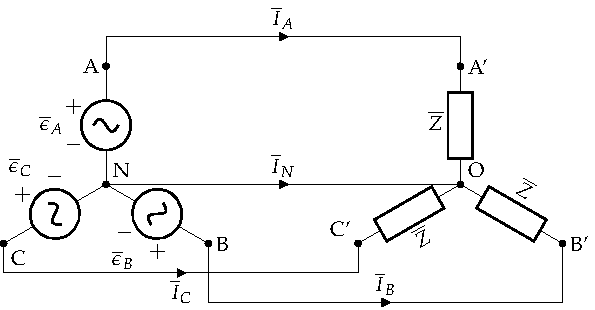
\includegraphics[width=.9\linewidth]{../figs/EstrellaEquilibrado.pdf}
    \end{center}
\end{frame}

%%%%%%%%%%%%%%%%%

\begin{frame}{Motivación de los sistemas trifásicos}

    \vspace{8mm}
    \begin{itemize}
    \item En un sistema trifásico la \alert{potencia instantánea es constante}, evitando vibraciones y esfuerzos en las máquinas 

    \vspace{2mm}
    \begin{itemize}
        \item \normalsize \alert{Recordatorio}: en un sistema monofásico, la potencia instantánea es pulsante
    \end{itemize}    

    \vspace{6mm}
    \item La \alert{masa de conductor necesaria} en un sistema trifásico \alert{es un 25\% inferior} que en un sistema monofásico para transportar la misma potencia
    \end{itemize}

    \vspace{2mm}
    
    \noindent\rule{\textwidth}{0.5pt}

    \vspace{2mm}

    \begin{center}
        Por estas razones, se usan sistemas trifásicos en \alert{generación,} 

        \vspace{-2mm}
        \alert{transporte y distribución de energía eléctrica}

        \vspace{1mm}
        \small{(los sistemas monofásicos se utilizan en cargas domésticas y de baja potencia)}
    \end{center}    
\end{frame}

%%%%%%%%%%%%%%%%%

\begin{frame}{Ondas trifásicas}
    \vspace{3mm}

    Para conseguir potencia constante, las ondas trifásicas deben cumplir:

    \vspace{1mm}
    \begin{itemize}
        \item Mismo \alert{desfase entre ellas} $\; \rightarrow \;$ el desfase debe ser de ${\boldsymbol{\color{blue!50!black} 120^\circ}}$

        \vspace{2mm}
        \item Igual \alert{amplitud}
    \end{itemize}

    \vspace{5mm}
    \begin{columns}
    \begin{column}{0.67\columnwidth}
        \hspace*{4mm}
        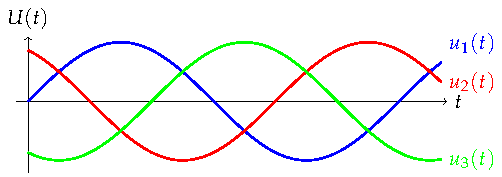
\includegraphics[width=1.05\linewidth]{../figs/TensionesTrifasica.pdf}
    \end{column}    
    \begin{column}{0.33\columnwidth}
        \vspace{-0.1mm}
        \begin{align*}
          &= U_0 \sin(\omega t)\\[7pt]
          &= U_0 \sin(\omega t + 2\pi/3)\\[10.8mm]
          &= U_0 \sin(\omega t - 2\pi/3)
        \end{align*}
    \end{column}
    \end{columns}
\end{frame}

%%%%%%%%%%%%%%%%%

\begin{frame}{Fasores de un sistema trifásico}
    \vspace{1mm}
    
    Usamos las mismas herramientas matemáticas que en el Tema 2 $\; \rightarrow \;$ \alert{cálculo fasorial}
    

    \vspace{8mm}
    \begin{columns}
    \begin{column}{0.35\columnwidth}
        \hspace*{35mm}
            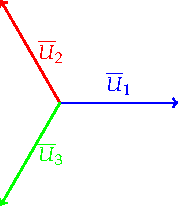
\includegraphics[height=0.5\textheight]{../figs/FasoresTrifasica.pdf}
    \end{column}    
    \begin{column}{0.65\columnwidth}
        \vspace{-0.1mm}
        \begin{align*}
          \overline{U}_1 &= U\phase{0}\\[4pt]
          \overline{U}_2 &= U\phase{2\pi/3}\\[4pt]
          \overline{U}_3 &= U\phase{-2\pi/3}
        \end{align*}
    \end{column}
    \end{columns}
\end{frame}

%%%%%%%%%%%%%%%%%

\begin{frame}{Generador trifásico}
    \begin{center}
        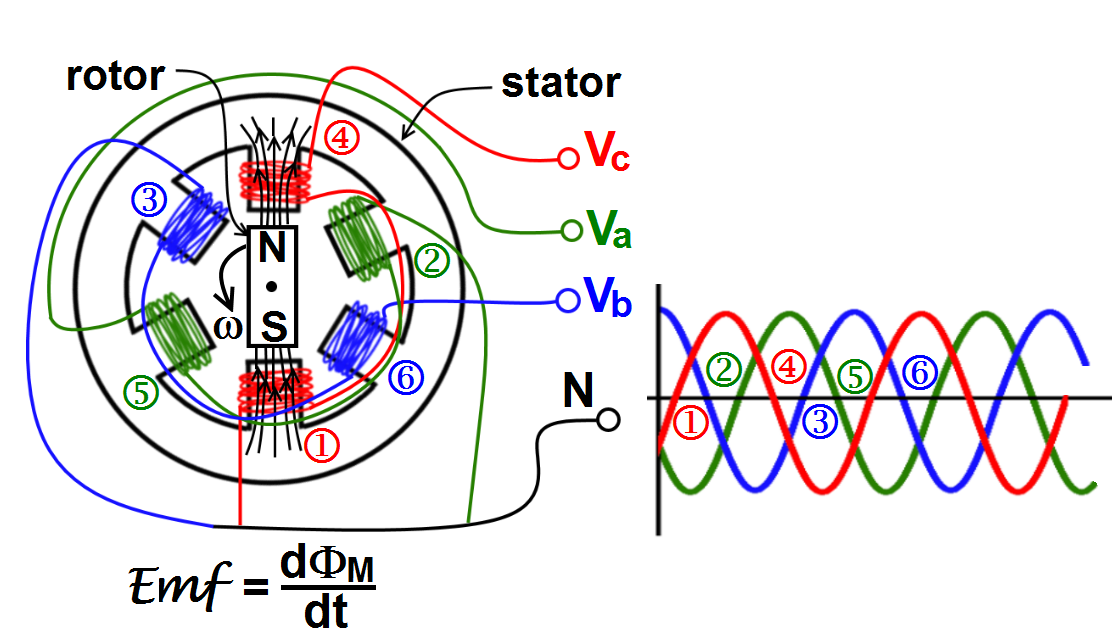
\includegraphics[width=.7\linewidth]{../figs/generador_trifasico.png}
    \end{center}
\end{frame}

%%%%%%%%%%%%%%%%%

\begin{frame}{}
    \vspace{2mm}
    (\alert{clica en la imagen})

    \vspace{2mm}
    \begin{center}
        \animategraphics[loop,width=11cm]{5}{../figs/gifs/gen_trifasica-}{0}{23}
    \end{center}
    % Info para insertar .gif: https://latex-beamer.com/tutorials/gif-latex-beamer/
    % Esta info también está en "figs\insert_GIF_Beamer.pdf"
\end{frame}

%%%%%%%%%%%%%%%%%

\begin{frame}{¿Por qué 3 fases?}

    ¿Por qué no 2, 5 o 17?
    
    \vspace{6mm}
    
    \begin{itemize}
        \item 2 fases 
        \begin{itemize}
            \vspace{2mm}
            \item \normalsize Requiere \alert{mayor masa de conductor} que un sistema trifásico
            
            %\vspace{2mm}
            %\item Aunque los sistemas bifásicos también proveen potencia constante, en la práctica los \alert{motores bifásicos pueden sufrir pulsaciones} 
            % % https://en.wikipedia.org/wiki/Two-phase_electric_power
            %
            % % Los sitemas bifásicos, tienen un desfase de 90º. Pág 29 del libro "Sistemas polifásicos": "un sistema bifásico no es puramente polifásico". La explicación es más extensa en la pág. 38.
        \end{itemize}

        \vspace{4mm}
        \item Más de 3 fases

        \vspace{2mm}
        \begin{itemize}  
            \item \normalsize El rendimiento de un motor o generador aumenta ligeramente con el nº de fases 

            \vspace{2mm}
            Pero la leve mejoría para más de 3 fases \alert{no justifica la mayor complejidad} del sistema (por ejemplo, las protecciones eléctricas serían bastante más complejas)  
        \end{itemize}
    \end{itemize}
\end{frame}

%%%%%%%%%%%%%%%%%

\section{Generadores}

\begin{frame}{Conexión}

    \begin{itemize}
        \item Punto común de la conexión estrella $\; \rightarrow \;$ \alert{neutro}, $N$
        \item Potencial de $N$ se toma como \alert{referencia}
    \end{itemize}

    \begin{center}
        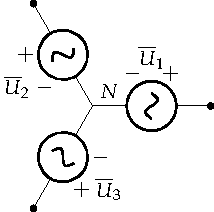
\includegraphics[height=0.5\textheight]{../figs/GeneradoresTrifasica.pdf}
    \end{center}

    \vspace{-12mm}
    \begin{columns}
    \begin{column}{0.45\columnwidth}
        \begin{align*}
          u_1(t) &= U_0 \sin(\omega t)\\[4pt]
          u_2(t) &= U_0 \sin(\omega t + 2\pi/3)\\[4pt]
          u_3(t) &= U_0 \sin(\omega t - 2\pi/3)
        \end{align*}
    \end{column}
    \hfill
    \begin{column}{0.5\columnwidth}
        \begin{align*}
          \overline{U}_1 &= U\phase{0}\\[4pt]
          \overline{U}_2 &= U\phase{2\pi/3}\\[4pt]
          \overline{U}_3 &= U\phase{-2\pi/3}
        \end{align*}
    \end{column}
    \end{columns}
\end{frame}

%%%%%%%%%%%%%%%%%

\begin{frame}{Las tensiones suman 0} \label{diapo:sumaFasores_Cero}
    \begin{center}
        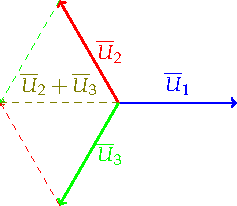
\includegraphics[height=0.6\textheight]{../figs/FasoresSumaCero.pdf}
    \end{center}
    
    \[
        \boxed{\overline{U}_1 + \overline{U}_2 + \overline{U}_3 = 0}
    \]
\end{frame}

%%%%%%%%%%%%%%%%%

\begin{frame}{Las tensiones suman 0}
    \vspace{2mm}
    \begin{center}
        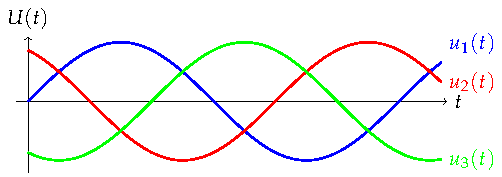
\includegraphics[width=.8\linewidth]{../figs/TensionesTrifasica.pdf}
    \end{center}
    
    \[
        \boxed{u_1(t) + u_2(t) + u_3(t) = 0}
    \]

    \vspace{4mm}
    \begin{center}
        \small{(esto no quiere decir que una carga vaya a estar sometida constantemente a \qty{0}{\volt}, porque 

        \vspace{-1mm}
        \alert{ninguna carga} va a estar \alert{sometida a las 3 tensiones} de fase a la vez)}
    \end{center}
    
\end{frame}

%%%%%%%%%%%%%%%%%

\begin{frame}{Tensiones de fase y de línea} \label{diapo:triangulos_fase_linea}

\vspace{7mm}
    \begin{columns}
    \begin{column}{0.35\columnwidth}
        \hspace*{8mm}
            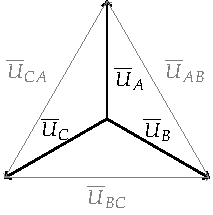
\includegraphics[height=0.5\textheight]{../figs/FasoresTrifasica_ABC.pdf}
    \end{column}
    
    \begin{column}{0.65\columnwidth}

        \vspace{-6mm}
        \begin{itemize}
            \item Tensiones de \alert{fase}: \hspace{4mm}\(U_A\), \(U_B\), \(U_C\) \hspace{1mm} $\equiv \;\, U_f$

            \vspace{1mm}
            \small{(o tensiones \alert{simples}, entre fase y neutro)}
    
            \normalsize
            \vspace{5mm}
            \item Tensiones de \alert{línea}: \hspace{1.5mm} \(U_{AB}\), \(U_{BC}\), \(U_{CA}\) \hspace{1mm} $\equiv \;\, U_L$
    
            \vspace{1mm}
            \small{(o tensiones \alert{compuestas}, entre dos conductores de línea)}
    
            \normalsize
        \end{itemize}        
    \end{column}
    \end{columns}

    \vspace{-5mm}
     \begin{align*}
       \overline{U}_{AB} &= \overline{U}_A - \overline{U}_B\\
       \overline{U}_{BC} &= \overline{U}_B - \overline{U}_C\\
       \overline{U}_{CA} &= \overline{U}_C - \overline{U}_A\\[-4pt]
    \cline{1-2}
       \overline{U}_{AB} + \overline{U}_{BC} + \overline{U}_{CA} &= 0    
    \end{align*}
\end{frame}

%%%%%%%%%%%%%%%%%

\begin{frame}{Relación entre tensiones de fase y de línea}
    \begin{columns}
    \begin{column}{0.5\columnwidth}
        \vspace{6mm}
        \begin{align*}
          \overline{U}_A &= U_f\phase{\theta_f}\\
          \overline{U}_B &= U_f\phase{\theta_f - \ang{120}}
        \end{align*}

        \vspace{-2mm}
        \begin{align*}
        \overline{U}_{AB} &= \overline{U}_A - \overline{U}_B = \\[-10pt]
        		   &= U_f\phase{\theta_f} - U_f\phase{\theta_f - \ang{120}} \overarrow[=][\downarrow]{\footnotesize {$\qquad\quad\; -\overline{A} = A\phase{\theta+\ang{180}}$}\vspace*{-1mm}} \\
        		  &= U_f\phase{\theta_f} + U_f\phase{\theta_f + \ang{60}} \overarrow[=][\downarrow]{\hspace*{10mm} \footnotesize ver gráfico\vspace*{-1mm}}\\[-11pt]
        		  &= 2 \cdot U_f \cdot \cos(\ang{30}) \phase{\theta_f + \ang{30}} \overarrow[=][\downarrow]{\footnotesize {\qquad\qquad\qquad $\cos(\ang{30})=\sqrt{3}/2$}\vspace*{-1mm}} \\[4pt]
          &= \sqrt{3} \; U_f \phase{\theta_f + \ang{30}}
        \end{align*}
    \end{column}
    
    \begin{column}{0.5\columnwidth}
    \begin{center}
    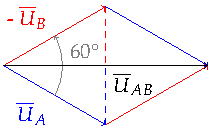
\includegraphics[width=.65\linewidth]{../figs/FasoresFaseLinea.pdf}
    \end{center}
    
    \[
      \large{\boxed{
        \begin{array}{l}
          U_L = \sqrt{3}\cdot U_f\\[4pt]
          \theta_L = \theta_f + \ang{30}\\
        \end{array}
      }}
    \]
    \end{column}
    \end{columns}
\end{frame}

%%%%%%%%%%%%%%%%%

\begin{frame}{Secuencia de fases} \label{diapo:secuencias_fases}
    \vspace{2mm}
    Orden en que ocurren los máximos de cada fase
    \begin{itemize}
        \item Secuencia de Fases Directa (\alert{SFD}): \hspace{3mm}ABC
    \end{itemize}

    \vspace{-3mm}
    \begin{center}
        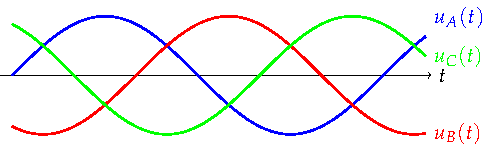
\includegraphics[height=0.34\textheight]{../figs/TensionesTrifasica_ABC.pdf}
    \end{center}

    \vspace{-2mm}
    \begin{itemize}
        \item Secuencia de Fases Inversa (\alert{SFI}): \hspace{5mm}ACB
    \end{itemize}

    \vspace{-3mm}
    \begin{center}
        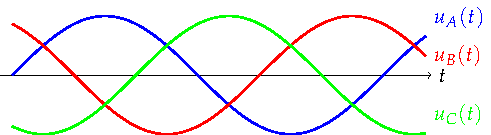
\includegraphics[height=0.305\textheight]{../figs/TensionesTrifasica_ACB.pdf}
    \end{center}
\end{frame}

%%%%%%%%%%%%%%%%%

\begin{frame}{Secuencia de Fases Directa (SFD)} \label{diapo:triangulo_SFD}

    \vspace{3mm}
    Por \alert{convenio}, se usa siempre esta \alert{referencia} de fases (\underline{memorizad} este triángulo):

    \begin{center}
        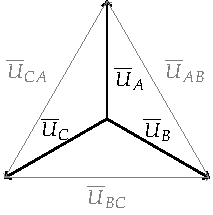
\includegraphics[height=0.56\textheight]{../figs/FasoresTrifasica_ABC.pdf}
    \end{center}

    \vspace{-10mm}
    \begin{columns}
    \begin{column}{0.5\columnwidth}
        \begin{align*}
          \overline{U}_A &= U_f \, \phase{{\color{blue}\ang{90}}}\\[4pt]
          \overline{U}_B &= U_f \, \phase{\ang{-30}}\\[4pt]
          \overline{U}_C &= U_f \, \phase{\ang{-150}}
        \end{align*}
    \end{column} 
    \begin{column}{0.5\columnwidth}
        \begin{align*}
          \overline{U}_{AB} &= U_L \, \phase{\ang{120}}\\[4pt]
          \overline{U}_{BC} &= U_L \, \phase{{\color{blue}\ang{0}}}\\[4pt]
          \overline{U}_{CA} &= U_L \, \phase{\ang{-120}}
        \end{align*}
    \end{column}
    \end{columns}

    %\begin{columns}
    %\begin{column}{0.35\columnwidth}
    %    \begin{align*}
    %      \overline{U}_A &= U_f \, \phase{{\color{blue}\ang{90}}}\\[4pt]
    %      \overline{U}_B &= U_f \, \phase{\ang{-30}}\\[4pt]
    %      \overline{U}_C &= U_f \, \phase{\ang{-150}}
    %    \end{align*}
    %\end{column}
    %\begin{column}{0.30\columnwidth}
    %    \begin{block}{Relación $U_f$ - $U_L$ en SFD}
    %        \begin{equation*}
    %    		\boxed{
    %    			\begin{array}{l}
    %    				U_L = \sqrt{3}\cdot U_f\\
    %    				\theta_L = \theta_f + 30^\circ\\
    %    			\end{array}
    %    		} 
    %    	\end{equation*}
    %    \end{block}
    %\end{column}    
    %\begin{column}{0.35\columnwidth}
    %    \begin{align*}
    %      \overline{U}_{AB} &= U_L \, \phase{\ang{120}}\\[4pt]
    %      \overline{U}_{BC} &= U_L \, \phase{{\color{blue}\ang{0}}}\\[4pt]
    %      \overline{U}_{CA} &= U_L \, \phase{\ang{-120}}
    %    \end{align*}
    %\end{column}
    %\end{columns}
\end{frame}

%%%%%%%%%%%%%%%%%

\begin{frame}{Secuencia de Fases Inversa (SFI)}

    \vspace{3mm}
    Por \alert{convenio}, se usa siempre esta \alert{referencia} de fases (\underline{memorizad} este triángulo):

    \vspace{3mm}
    \begin{center}
        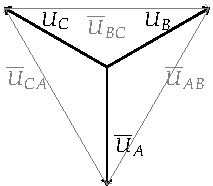
\includegraphics[height=0.49\textheight]{../figs/FasoresTrifasica_ACB.pdf}
    \end{center}

    \vspace{-6mm}
    \begin{columns}
    \begin{column}{0.5\columnwidth}
        \begin{align*}
          \overline{U}_A &= U_f \, \phase{{\color{blue}\ang{-90}}}\\[4pt]
          \overline{U}_B &= U_f \, \phase{\ang{30}}\\[4pt]
          \overline{U}_C &= U_f \, \phase{\ang{150}}
        \end{align*}
    \end{column}   
    \begin{column}{0.5\columnwidth}
        \begin{align*}
          \overline{U}_{AB} &= U_L \, \phase{\ang{-120}}\\[4pt]
          \overline{U}_{BC} &= U_L \, \phase{{\color{blue}\ang{0}}}\\[4pt]
          \overline{U}_{CA} &= U_L \, \phase{\ang{120}}
        \end{align*}
    \end{column}
    \end{columns}

    %\begin{columns}
    %\begin{column}{0.35\columnwidth}
    %    \begin{align*}
    %      \overline{U}_A &= U_f \, \phase{{\color{blue}\ang{-90}}}\\[4pt]
    %      \overline{U}_B &= U_f \, \phase{\ang{30}}\\[4pt]
    %      \overline{U}_C &= U_f \, \phase{\ang{150}}
    %    \end{align*}
    %\end{column}    
    %\begin{column}{0.30\columnwidth}
    %    \begin{block}{Relación $U_f$ - $U_L$ en SFI}
    %        \begin{equation*}
    %    		\boxed{
    %    			\begin{array}{l}
    %    				U_L = \sqrt{3}\cdot U_f\\
    %    				\theta_L = \theta_f - 30^\circ\\
    %    			\end{array}
    %    		} 
    %    	\end{equation*}
    %    \end{block}
    %\end{column}
    %\begin{column}{0.35\columnwidth}
    %    \begin{align*}
    %      \overline{U}_{AB} &= U_L \, \phase{\ang{-120}}\\[4pt]
    %      \overline{U}_{BC} &= U_L \, \phase{{\color{blue}\ang{0}}}\\[4pt]
    %      \overline{U}_{CA} &= U_L \, \phase{\ang{120}}
    %    \end{align*}
    %\end{column}
    %\end{columns}
\end{frame}

%%%%%%%%%%%%%%%%%

%\begin{frame}{Secuencia de fases}{Secuencia de fases directa (SFD)}
%    \begin{columns}
%    \begin{column}{0.25\columnwidth}
%        \begin{center}
%        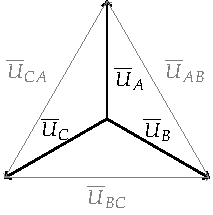
\includegraphics[width=\linewidth]{../figs/FasoresTrifasica_ABC.pdf}
%        \end{center}
%    \end{column}
%    \begin{column}{0.25\columnwidth}
%        \begin{align*}
%          \overline{U}_A &= U_f\phase{{\color{blue}\ang{90}}}\\
%          \overline{U}_B &= U_f\phase{\ang{-30}}\\
%          \overline{U}_C &= U_f\phase{\ang{-150}}
%    \end{align*}
%    \end{column}
%    \begin{column}{0.5\columnwidth}
%    	\begin{align*}
%    		&\overline{U}_{AB}=\overline{U}_{A}-\overline{U}_{B}=\\&=(0+\mathrm{j}\,U_f)-\left(\dfrac{\sqrt{3}\,U_f}{2}-\mathrm{j}\,\dfrac{U_f}{2}\right)=\\
%    		&=-\dfrac{\sqrt{3}\cdot U_f}{2}+\mathrm{j}\,\dfrac{3\,U_f}{2}=\sqrt{3}\,U_f \phase{ 120^\circ}
%    	\end{align*}
%    \end{column}
%    \end{columns}
%    
%    \begin{columns}
%    \begin{column}{0.2\columnwidth}
%        \begin{align*}
%          \overline{U}_A &= U_f\phase{{\ang{90}}}\\
%          \overline{U}_B &= U_f\phase{\ang{-30}}\\
%          \overline{U}_C &= U_f\phase{\ang{-150}}
%        \end{align*}
%    \end{column}
%    \begin{column}{0.2\columnwidth}
%        \begin{align*}
%          \overline{U}_{AB} &= \sqrt{3}\,U_f\phase{\ang{120}}\\
%          \overline{U}_{BC} &= \sqrt{3}\,U_f\phase{\ang{0}}\\
%          \overline{U}_{CA} &= \sqrt{3}\,U_f\phase{\ang{-120}}
%        \end{align*}
%    \end{column}
%    \begin{column}{0.4\columnwidth}
%        \begin{block}{Relación tensión fase-línea SFD}
%        	\begin{equation*}
%        		\boxed{
%        			\begin{array}{l}
%        				U_L = \sqrt{3}\cdot U_f\\
%        				\theta_L = \theta_f + 30^\circ\\
%        			\end{array}
%        		} 
%        	\end{equation*}
%        \end{block}
%    \end{column}
%    \end{columns}
%\end{frame}

%%%%%%%%%%%%%%%%%

%\begin{frame}{Secuencia de fases}{Secuencia de fases inversa (SFI)}
%    \begin{columns}
%    \begin{column}{0.25\columnwidth}
%        \begin{center}
%            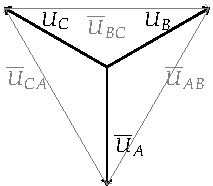
\includegraphics[width=\linewidth]{../figs/FasoresTrifasica_ACB.pdf}
%        \end{center}
%    \end{column}
%    \begin{column}{0.25\columnwidth}
%        \begin{align*}
%          \overline{U}_A &= U_f\phase{{\color{blue}\ang{-90}}}\\
%          \overline{U}_B &= U_f\phase{\ang{30}}\\
%          \overline{U}_C &= U_f\phase{\ang{150}}
%        \end{align*}
%    \end{column}
%    \begin{column}{0.5\columnwidth}
%    	\begin{align*}
%    		&\overline{U}_{AB}=\overline{U}_{A}-\overline{U}_{B}=\\&=(0-\mathrm{j}\,U_f)-\left(\dfrac{\sqrt{3}\,U_f}{2}+\mathrm{j}\,\dfrac{U_f}{2}\right)=\\
%    		&=-\dfrac{\sqrt{3}\cdot U_f}{2}-\mathrm{j}\,\dfrac{3\,U_f}{2}=\sqrt{3}\,U_f \phase{-120^\circ}
%    	\end{align*}
%    \end{column}
%    \end{columns}
%    
%    \begin{columns}
%    \begin{column}{0.2\columnwidth}
%        \begin{align*}
%          \overline{U}_A &= U_f\phase{{\ang{-90}}}\\
%          \overline{U}_B &= U_f\phase{\ang{30}}\\
%          \overline{U}_C &= U_f\phase{\ang{150}}
%        \end{align*}
%    \end{column}
%    \begin{column}{0.2\columnwidth}
%        \begin{align*}
%          \overline{U}_{AB} &= \sqrt{3}\,U_f\phase{\ang{-120}}\\
%          \overline{U}_{BC} &= \sqrt{3}\,U_f\phase{\ang{0}}\\
%          \overline{U}_{CA} &= \sqrt{3}\,U_f\phase{\ang{120}}
%        \end{align*}
%    \end{column}
%    \begin{column}{0.4\columnwidth}
%        \begin{block}{Relación tensión fase-línea SFI}
%        	\begin{equation*}
%        		\boxed{
%        			\begin{array}{l}
%        				U_L = \sqrt{3}\cdot U_f\\
%        				\theta_L = \theta_f - 30^\circ\\
%        			\end{array}
%        		} 
%        	\end{equation*}
%        \end{block}
%    \end{column}
%    \end{columns}
%\end{frame}

%%%%%%%%%%%%%%%%%

\section{Receptores}

\begin{frame}{Tipos de receptor}
    Según su \alert{conexión}:
    \vspace{1mm}
        \begin{itemize}
            \item \alert{Estrella} (punto común) 
            \vspace{2mm}
            \item \alert{Triángulo} 
        \end{itemize}

    \vspace{5mm}
    Según sus \alert{impedancias}:
    \vspace{1mm}
        \begin{itemize}
            \item \alert{Equilibrado} (las tres impedancias son idénticas en \underline{módulo} y \underline{fase})
            \vspace{2mm}
            \item \alert{Desequilibrado}
        \end{itemize}
\end{frame}

%%%%%%%%%%%%%%%%%

\begin{frame}{Receptor en estrella equilibrado, \hspace{3mm}con neutro}
    \begin{center}
        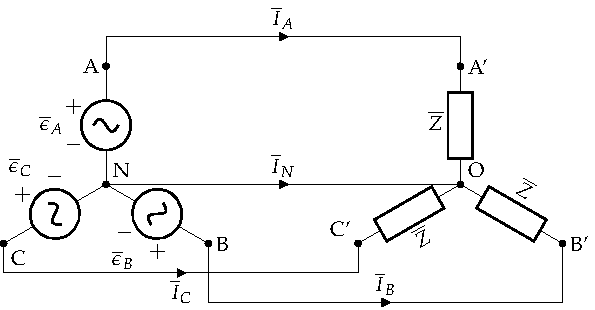
\includegraphics[width=.9\linewidth]{../figs/EstrellaEquilibrado.pdf}
    \end{center}
\end{frame}
    
%%%%%%%%%%%%%%%%%

\begin{frame}{Receptor en estrella equilibrado, \hspace{3mm}con neutro}
    \begin{columns}
    \begin{column}{0.5\columnwidth}
        \begin{center}
            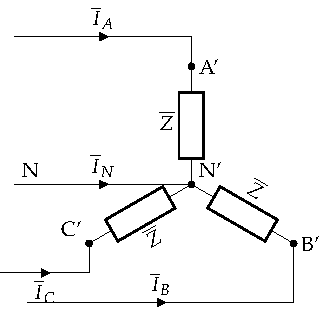
\includegraphics[width=.9\linewidth]{../figs/EstrellaEquilibrado_Receptor.pdf}
        \end{center}
    \end{column}
    
    \begin{column}{0.5\columnwidth}
        \begin{columns}
        \begin{column}{0.5\columnwidth}
            \begin{align*}
              \overline{I}_A &= \frac{\overline{U}_A}{\overline{Z}} = \frac{U_f}{Z}\phase{\ang{\pm 90} - \theta} \\
              \overline{I}_B &= \frac{\overline{U}_B}{\overline{Z}} = \frac{U_f}{Z}\phase{\ang{\mp 30} - \theta}\\
              \overline{I}_C &= \frac{\overline{U}_C}{\overline{Z}} = \frac{U_f}{Z}\phase{\ang{\mp 150} - \theta}
            \end{align*}    
        \end{column}
        \begin{column}{0.5\columnwidth}
            \begin{center}
                \footnotesize{(signo de arriba 
                
                para \alert{SFD},
                
                signo de abajo 
                
                para \alert{SFI})}
            \end{center}
        \end{column}
        \end{columns}

        \vspace{3mm}
        \[
          \boxed{I_A = I_B = I_C = \frac{U_f}{Z}}
        \]
        \begin{center}
            \small{(en \wye, corriente de línea igual a la de fase)}
        \end{center}

        \small{Aplicando \alert{1LK} en el punto común del receptor:}
        \normalsize     
        \vspace{-1mm}
        \[
          \overline{I}_A  + \overline{I}_B + \overline{I}_C + \overline{I}_N = 0
        \]

        \vspace{-5mm}
        \[
           \overline{I}_A  + \overline{I}_B + \overline{I}_C  \hyperlink{diapo:sumaFasores_Cero}{= 0} \quad \rightarrow \quad \boxed{\overline{I}_N = 0}
        \]
        % Sobre la cross-reference usando "hyperlink": https://tex.stackexchange.com/questions/70143/cross-reference-with-custom-text
    \end{column}
    \end{columns}
\end{frame}

%%%%%%%%%%%%%%%%%

\begin{frame}{Receptor en estrella equilibrado, \hspace{3mm}sin neutro}
    \begin{columns}
    \begin{column}{0.79\columnwidth}
        \vspace{-21mm}

        \hspace*{0mm}
        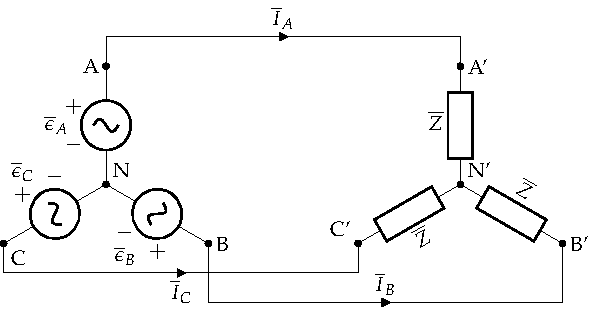
\includegraphics[width=1.21\linewidth]{../figs/EstrellaEquilibrado_SinNeutro.pdf}
    
        \vspace{-58mm}
        
        \hspace*{32mm}
        \small{Dado que no circulaba corriente por el neutro,}

        \vspace{-3mm}
        \hspace*{38mm}
        \small{se puede \alert{prescindir} de este conductor}
        \LARGE{
        \[
            \qquad\quad  {\color{blue!50!black} \overline{U}_N = \overline{U}_{N'} }
        \]
        }
    \end{column}
    \begin{column}{0.21\columnwidth}
        \vspace*{-45mm}
        \footnotesize{
        \begin{center}
            Al igual que en $Z_{\wye}$ con neutro, se cumple:
        \end{center}    
        \[
          I_A = I_B = I_C = \frac{U_f}{Z}
        \]
        \[
          \overline{I}_A  + \overline{I}_B + \overline{I}_C = 0
        \]
        }
    \end{column}
    \end{columns}
\end{frame}

%%%%%%%%%%%%%%%%%

\begin{frame}{Ejercicio}
    \vspace{19mm}
    Un sistema a cuatro hilos y SFI alimenta tres impedancias $\overline{Z}=10\phase{60^\circ}\,\Omega$, conectadas en estrella a una tensión de $200\sqrt{3}$ \si{\volt} 

    \vspace{5mm}
    Determinar las corrientes de línea y el diagrama fasorial

    \vspace{28mm}
    \alert{Solución}: \href{https://raw.githubusercontent.com/ETSIDI-IE/tc/master/docs/ejercicios_clase/TC1_03_Ejemplo_3_1_libro_LBB.pdf}{aquí}
\end{frame}

%%%%%%%%%%%%%%%

\begin{frame}{Receptor en estrella equilibrado, \hspace{3mm}con carga monofásica}
    \begin{columns}
    \begin{column}{0.8\columnwidth}
        \vspace{3mm}
        
        \hspace*{9mm}
        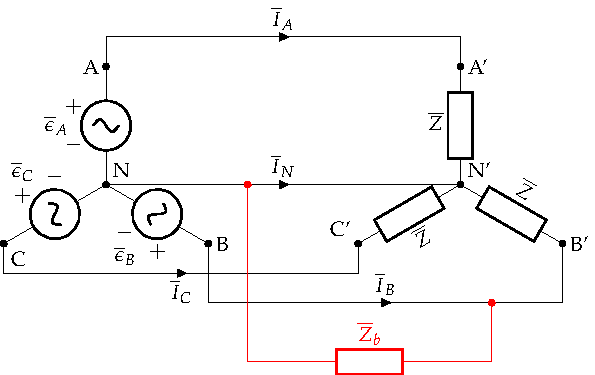
\includegraphics[height=0.9\textheight]{../figs/Estrella_CargaMonofasica.pdf}
    \end{column}
    \begin{column}{0.2\columnwidth}
        \vspace{-40mm}
        \begin{center}
            \footnotesize{(para $Z_{\wye}$ equilibrado, se incluye neutro cuando convive con cargas monofásicas, \textit{e.g.}~edificios)}
        \end{center}
    \end{column}
    \end{columns}    
\end{frame}

%%%%%%%%%%%%%%%%%

\begin{frame}{Receptor en triángulo equilibrado}
    \begin{center}
        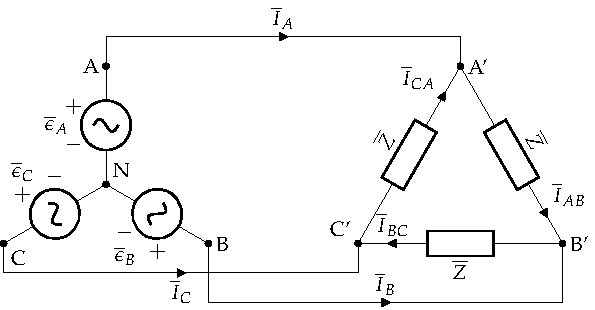
\includegraphics[width=.9\linewidth]{../figs/TrianguloEquilibrado.pdf}
    \end{center}
\end{frame}

%%%%%%%%%%%%%%%%%

\begin{frame}{Receptor en triángulo equilibrado}
    \begin{columns}
    \begin{column}{0.5\columnwidth}
            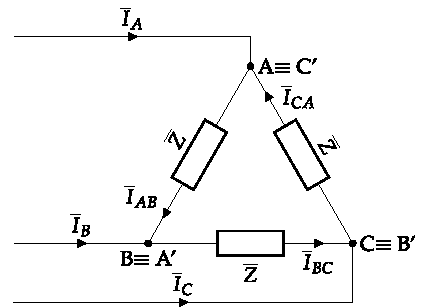
\includegraphics[width=.9\linewidth]{../figs/TrianguloEquilibrado_Receptor.pdf}
    \end{column}
    
    \begin{column}{0.5\columnwidth}
        \vspace{-2mm}
        \begin{columns}
        \begin{column}{0.5\columnwidth}
            \begin{align*}
              \overline{I}_{AB} &= \frac{\overline{U}_{AB}}{\overline{Z}} = \frac{U_L}{Z}\phase{\ang{\pm 120} - \theta} \\[2pt]
              \overline{I}_{BC} &= \frac{\overline{U}_{BC}}{\overline{Z}} = \frac{U_L}{Z}\phase{0 - \theta}\\[2pt]
              \overline{I}_{CA} &= \frac{\overline{U}_{CA}}{\overline{Z}} = \frac{U_L}{Z}\phase{\ang{\mp 120} - \theta}
            \end{align*}
        \end{column}
        \begin{column}{0.5\columnwidth}
            \begin{center}
                \footnotesize{(signo de arriba 
                
                para \alert{SFD},
                
                signo de abajo 
                
                para \alert{SFI})}
            \end{center}
        \end{column}
        \end{columns}

        \begin{center}
            \small{(en $\triangle$, tensión de línea igual a la de fase)}
        \end{center}

        \vspace{1mm}
        
        \hspace*{-5mm}\small{Por la misma razón que en la diapositiva~\ref{diapo:sumaFasores_Cero}:}
        \normalsize

        \vspace{-3mm}
        \[
           \overline{I}_{AB}  + \overline{I}_{BC} + \overline{I}_{CA}  = 0 
        \]

        \vspace{1mm}
        Corriente de \alert{fase}:
        \[
          \boxed{I_f = {I}_{AB} = {I}_{BC} = {I}_{CA} = \frac{U_L}{Z}}
        \]
    \end{column}
    \end{columns}
\end{frame}

%%%%%%%%%%%%%%%%%

\begin{frame}{Receptor en triángulo equilibrado}
    \begin{columns}
    \begin{column}{0.5\columnwidth}
            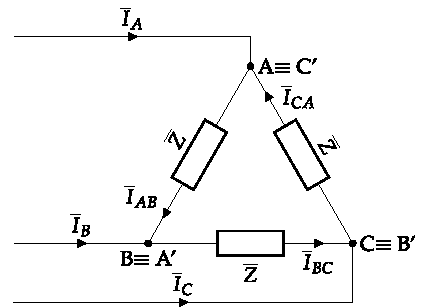
\includegraphics[width=.9\linewidth]{../figs/TrianguloEquilibrado_Receptor.pdf}
    \end{column}
    
    \begin{column}{0.5\columnwidth}
        
        \vspace{3mm}
        \small{Para calcular las corrientes de línea,} 
        
        \small{aplicamos \alert{1LK} en cada nudo:}

        \vspace{-3mm}
        \begin{align*}
          \overline{I}_A &= \overline{I}_{AB} - \overline{I}_{CA} = \sqrt{3} \cdot \frac{U_L}{Z}\phase{\ang{\pm 90} - \theta}\\
          \overline{I}_B &= \overline{I}_{BC} - \overline{I}_{AB} = \sqrt{3} \cdot \frac{U_L}{Z}\phase{\ang{\mp 30} - \theta}\\
          \overline{I}_C &= \overline{I}_{CA} - \overline{I}_{BC} = \sqrt{3} \cdot \frac{U_L}{Z}\phase{\ang{\mp 150} - \theta}\\
        \end{align*}
        
        \normalsize
        \vspace{-3mm}
        Corriente de \alert{línea}:
        \[
          \boxed{I_L = {I}_A = {I}_B = {I}_C = \sqrt{3} \cdot \frac{U_L}{Z}}
        \]

        \vspace{-2mm}
        \[
          \boxed{I_L = \sqrt{3} \cdot I_f}
        \]
    \end{column}
    \end{columns}
\end{frame}

%%%%%%%%%%%%%%%%%

\begin{frame}{Ejercicio}
    \vspace{19mm}
    Un sistema trifásico de secuencia directa y tensión $\qty{200}{\volt}$ alimenta tres impedancias iguales $\overline{Z}=10\phase{30^\circ}\,\Omega$, conectadas en triángulo

    \vspace{5mm}
    Determinar las corrientes de fase y línea, y dibujar el diagrama fasorial

    \vspace{28mm}
    \alert{Solución}: \href{https://raw.githubusercontent.com/ETSIDI-IE/tc/master/docs/ejercicios_clase/TC1_03_Ejemplo_3_3_libro_LBB.pdf}{aquí}
\end{frame}

%%%%%%%%%%%%%%%

\begin{frame}{Receptor en estrella desequilibrado, \hspace{3mm}con neutro}

    \vspace{2mm}
    Si cada una de las impedancias es distinta, el receptor es \alert{desequilibrado}

    \vspace{-2mm}
    \begin{center}
        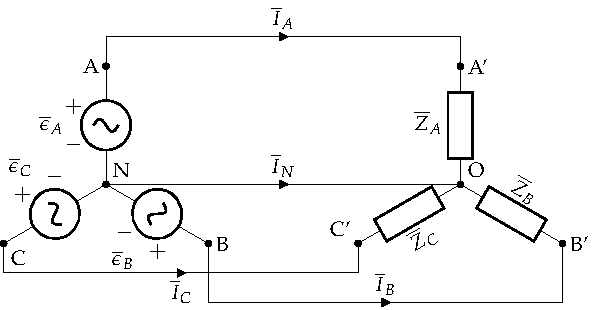
\includegraphics[width=.9\linewidth]{../figs/EstrellaDesequilibrado.pdf}
    \end{center}
\end{frame}

%%%%%%%%%%%%%%%%%

\begin{frame}{Receptor en estrella desequilibrado, \hspace{3mm} con neutro}
    \begin{columns}
    \begin{column}{0.5\columnwidth}
        \begin{center}
            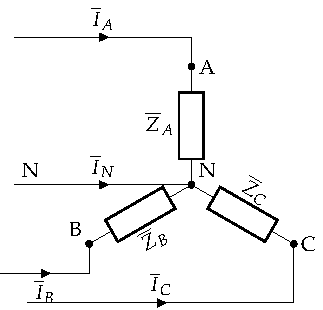
\includegraphics[width=.9\linewidth]{../figs/EstrellaDesequilibrado_Receptor.pdf}
        \end{center}
    \end{column}
    
    \begin{column}{0.5\columnwidth}
        \begin{align*}
          \overline{I}_A &= \frac{\overline{U}_A}{\overline{Z}_{\color{red}{A}}}\\[6pt]
          \overline{I}_B &= \frac{\overline{U}_B}{\overline{Z}_{\color{red}{B}}}\\[6pt]
          \overline{I}_C &= \frac{\overline{U}_C}{\overline{Z}_{\color{red}{C}}}
        \end{align*}

        \begin{center}
            \footnotesize{(cada corriente de fase/línea es \alert{distinta})}
        \end{center}
        
        \vspace{2mm}
        \small{Aplicando \alert{1LK} en el punto común del receptor:}
        \vspace{1mm}
        \[
          \overline{I}_A  + \overline{I}_B + \overline{I}_C + \overline{I}_N = 0
        \]

        \vspace{-3mm}
        \[
           \overline{I}_A  + \overline{I}_B + \overline{I}_C  \neq 0 \quad \rightarrow \quad \boxed{\overline{I}_N \; {\color{red} \neq} \; 0}
        \]
    \end{column}
    \end{columns}
\end{frame}

%%%%%%%%%%%%%%%%%

\begin{frame}{Receptor en estrella desequilibrado, \hspace{3mm} sin neutro}
    \vspace{-29mm}
    \begin{center}
        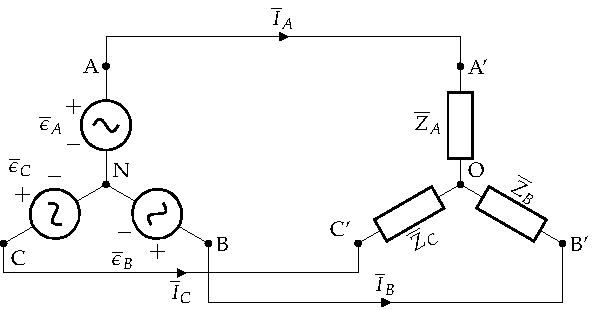
\includegraphics[width=.95\linewidth]{../figs/EstrellaDesequilibrado_SinNeutro.pdf}
    \end{center}
    
    \vspace{-65mm}
    
    \hspace*{41mm}
    \small{Los neutros de generador y receptor}

    \vspace{-1mm}
    
    \hspace*{37mm}
    \small{generalmente \alert{NO} están al mismo potencial}
    
    \LARGE{
    \(
        \qquad\qquad\qquad\qquad\qquad
        {\color{blue!50!black} \overline{U}_N} {\color{red} \neq } {\color{blue!50!black} \overline{U}_{N'} }
    \)
    % Si N y N' estuvieran al mismo potencial, al cortocircuitar esos puntos no circularía corriente por el cortocircuito, pero hemos visto en la diapositiva anterior que si ponemos neutro (que es equivalente a cortocircuitar esos puntos), SÍ que circularía corriente, lo que implica que esos puntos no están al mismo potencial.
    }
\end{frame}

%%%%%%%%%%%%%%%%%

\begin{frame}{Receptor en estrella desequilibrado, \hspace{3mm} sin neutro}

    \vspace{2mm}
    En este caso \alert{desconocemos la tensión} en las impedancias

    \begin{itemize}
        \item Podría resolverse el circuito por el \alert{método de las mallas}
    \end{itemize} 

    \vspace{-1mm}
    \begin{center}
        \includegraphics[width=.85\linewidth]{../figs/EstrellaDesequilibrado_SinNeutro_Mallas.pdf}
    \end{center}    
\end{frame}

%%%%%%%%%%%%%%%%%

\begin{frame}{Ejercicio}
    \vspace{19mm}
    Un sistema trifásico de cuatro conductores, de secuencia de fases directa y $\SI[parse-numbers=false]{200\sqrt{3}}{\volt}$ alimenta a tres impedancias: $\overline{Z}_{A} = {10\phase{\ang{60}}}\unit{\ohm}$, $\overline{Z}_{B} = {10\phase{\ang{0}}}\unit{\ohm}$ y $\overline{Z}_{C} = {10\phase{\ang{-30}}}\unit{\ohm}$  

    \vspace{5mm}
    Determinar las corrientes de línea

    \vspace{28mm}
    \alert{Solución}: \href{https://raw.githubusercontent.com/ETSIDI-IE/tc/master/docs/ejercicios_clase/TC1_03_Ejemplo_3_2_libro_LBB.pdf}{aquí}
\end{frame}

%%%%%%%%%%%%%%%

\begin{frame}{Receptor en triángulo desequilibrado}
    \begin{center}
        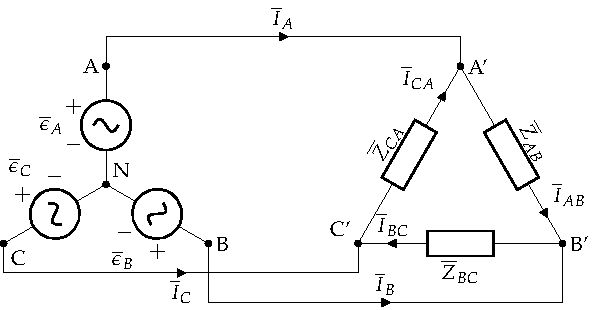
\includegraphics[height=0.85\textheight]{../figs/TrianguloDesequilibrado.pdf}
    \end{center}
\end{frame}

%%%%%%%%%%%%%%%%%

\begin{frame}{Receptor en triángulo desequilibrado}
    \begin{columns}
    \begin{column}{0.6\columnwidth}
        \begin{center}
            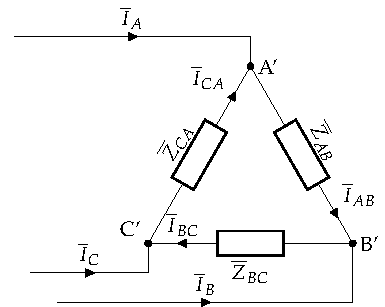
\includegraphics[width=.9\linewidth]{../figs/TrianguloDesequilibrado_Receptor.pdf}
        \end{center}
    \end{column}
    
    \begin{column}{0.4\columnwidth}
        \begin{align*}
          \overline{I}_{AB} &= \frac{\overline{U}_{AB}}{\overline{Z}_{\color{red}{AB}}}\\[4pt]
          \overline{I}_{BC} &= \frac{\overline{U}_{BC}}{\overline{Z}_{\color{red}{BC}}}\\[4pt]
          \overline{I}_{CA} &= \frac{\overline{U}_{CA}}{\overline{Z}_{\color{red}{CA}}}
        \end{align*}
        \begin{center}
            \footnotesize{(cada corriente de fase es \alert{distinta})}
        \end{center}        

        \vspace{-7mm}    
        \begin{align*}
          \overline{I}_A &= \overline{I}_{AB} - \overline{I}_{CA}\\
          \overline{I}_B &= \overline{I}_{BC} - \overline{I}_{AB}\\
          \overline{I}_C &= \overline{I}_{CA} - \overline{I}_{BC}\\
        \end{align*}

        \vspace{-9mm}   
        \begin{center}
            \footnotesize{(luego cada corriente de línea es \alert{distinta})}
        \end{center}
    \end{column}
    \end{columns}
\end{frame}

%%%%%%%%%%%%%%%

\begin{frame}{Ejercicio}
    \vspace{19mm}
    Un sistema trifásico de SFI y tensión $\qty{200}{\volt}$ alimenta tres impedancias conectadas en triángulo, de valor $\overline{Z}_{AB}=10\phase{0^\circ}\,\Omega$, $\overline{Z}_{BC}=10\phase{30^\circ}\,\Omega$ y $\overline{Z}_{CA}=10\phase{-45^\circ}\,\Omega$  

    \vspace{5mm}
    Determinar las corrientes de fase y línea, y dibujar el diagrama fasorial

    \vspace{28mm}
    \alert{Solución}: \href{https://raw.githubusercontent.com/ETSIDI-IE/tc/master/docs/ejercicios_clase/TC1_03_Ejemplo_3_4_libro_LBB.pdf}{aquí}
\end{frame}

%%%%%%%%%%%%%%%

\begin{frame}{Resumen}
    \vspace{0mm}
    \[
      \begin{array}{lcc}
        \text{Conexión del receptor} & \;\; \text{Tensiones} & \;\; \text{Corrientes}\\[5pt]
        \hline\\[-5pt]
        \text{\wye \hspace{1.5mm}equilibrado} & \quad \sqrt{3} \;U_f = U_L & \;\; I_f=I_L \\[10pt]
        \text{$\triangle$ equilibrado} & \quad U_f=U_L & \;\; \sqrt{3} \;I_f = I_L \\[10pt]
        \minibox[l]{\wye \hspace{1.5mm}desequilibrado, \\[-2pt] con neutro} \hspace*{13mm} & \quad \sqrt{3} \;U_f = U_L & \quad \minibox[c]{\small Deben calcularse  \\[-2pt] para cada impedancia} \\[15pt]
        \minibox[l]{\wye \hspace{1.5mm}desequilibrado, \\[-2pt] sin neutro} & \multicolumn{2}{c}{\smash{\raisebox{.2\normalbaselineskip}{\text{Resolución por método de las mallas}}}}
        \\[10pt] 
        \text{$\triangle$ desequilibrado} & \quad U_f=U_L & \quad \minibox[c]{\small Deben calcularse  \\[-2pt] para cada impedancia} \\[10pt]
        \hline
      \end{array}
    \]
    % "Minibox", para poder partir el texto en 2 líneas: https://tex.stackexchange.com/questions/8680/how-can-i-insert-a-newline-in-a-framebox
    % Sobre "\smash{\raisebox", sacado de aquí: https://tex.stackexchange.com/questions/153225/combining-rows-and-columns-in-array

    \vspace{2mm}   
    \begin{center}
        \small
        
        \alert{Nota}: $U_f$ en esta diapositiva se refiere a la tensión en cada \underline{fase del receptor}            

        \vspace{-1mm}         
        (tensión en cada impedancia), \alert{NO} a $U_f$ del \hyperlink{diapo:triangulos_fase_linea}{generador en estrella}
    \end{center}
\end{frame}

%%%%%%%%%%%%%%%%

\begin{frame}{Recordatorio del Tema 1: \hspace{3mm}conversión $\wye - \triangle$, \hspace{3mm}caso equilibrado}
    
    En el caso de receptores estrella/triángulo \alert{equilibrados}\ldots{}

    \vspace{-5mm}
    \begin{align*}
      \overline{Z}_A = \overline{Z}_B = \overline{Z}_C \; &= \; \overline{Z}_{\wye}\\[5pt]
      \overline{Z}_{AB} = \overline{Z}_{BC} = \overline{Z}_{CA} \; &= \; \overline{Z}_{\triangle}
    \end{align*}

    \vspace{2mm}
    \ldots{}la expresión para \alert{transformar} entre $\; \wye - \triangle \;$ es:
    
    \begin{equation*}
      \boxed{\;\, \vphantom{\frac{a}{a}} \overline{Z}_{\triangle} 
      \; = \; 
      3\cdot \overline{Z}_{\wye} \;\,}
    \end{equation*}
\end{frame}

%%%%%%%%%%%%%%%%%

\section{Potencia en sistemas trifásicos}

\begin{frame}{Potencia instantánea en sistemas equilibrados}
    Supongamos un \alert{receptor equilibrado} con \hyperlink{diapo:triangulo_SFD}{SFD} (la deducción es equivalente para SFI):     

    \vspace{2mm}
    \begin{columns}
    \begin{column}{0.5\columnwidth}
    \begin{align*}
      u_A(t) &= \sqrt{2} \, U_f \, \cos(\omega t + \pi/2)\\
      u_B(t) &= \sqrt{2} \, U_f \, \cos(\omega t - \pi/6)\\
      u_C(t) &= \sqrt{2} \, U_f \, \cos(\omega t - 5\pi/6)
    \end{align*}
    
    \begin{align*}
      i_A(t) &= \sqrt{2} \, I_f \, \cos(\omega t + \pi/2 - \theta)\\
      i_B(t) &= \sqrt{2} \, I_f \, \cos(\omega t - \pi/6 - \theta)\\
      i_C(t) &= \sqrt{2} \, I_f \, \cos(\omega t - 5\pi/6 - \theta)
    \end{align*}
    \end{column}
    
    \begin{column}{0.5\columnwidth}
    \begin{align*}
      p_A(t) &= u_A(t) \cdot i_A(t)\\
      p_B(t) &= u_C(t) \cdot i_B(t)\\
      p_C(t) &= u_C(t) \cdot i_C(t)\\
      \\
      p(t) &= p_A(t) + p_B(t) + p_C(t)
    \end{align*}
    \end{column}
    \end{columns}
\end{frame}

%%%%%%%%%%%%%%%%%

\begin{frame}{Potencia instantánea en sistemas equilibrados}
    \begin{align*}
      p(t) \;\; = \;\; &\sqrt{2}\, U_f \, \cos(\omega t + \pi/2) \cdot \sqrt{2}\, I_f\, \cos(\omega t + \pi/2 - \theta) +\\
           + &\sqrt{2}\, U_f \, \cos(\omega t - \pi/6) \cdot \sqrt{2}\, I_f \, \cos(\omega t - \pi/6 - \theta) +\\
           + &\sqrt{2}\, U_f \, \cos(\omega t - 5\pi/6) \cdot \sqrt{2}\, I_f \, \cos(\omega t - 5\pi/6 - \theta)
    \end{align*}
    \[
      \cos(\alpha) \cdot \cos(\beta) \; = \; \frac{1}{2} \cdot [\cos(\alpha + \beta) + \cos(\alpha - \beta)]
    \]
    \begin{align*}
      p(t) \;\; = \;\; &U_f \, I_f \, [{\color{gray}\cos(2 \omega t + \pi -\theta)} + \cos(\theta)] +\\
           + &U_f \, I_f \, [{\color{gray}\cos(2 \omega t - \pi/3 - \theta)} + \cos(\theta)] +\\
           + &U_f \, I_f \, [{\color{gray}\cos(2 \omega t - 5\pi/3 - \theta)} + \cos(\theta)]
    \end{align*}
    \begin{center}
        (los términos en {\color{gray}gris} suman cero, recordad \hyperlink{diapo:sumaFasores_Cero}{esta} propiedad)
    \end{center}
    \[
      \boxed{\quad p(t) \; = \; 3 \cdot U_f \cdot I_f \cdot \cos (\theta) \; = \; \sqrt3 \cdot U_L \cdot I_L \cdot \cos (\theta) \quad}
    \]
    % Esta expresión es válida para cargas tanto en estrella como en triángulo, tanto SFD como SFI. Pero solo vale para sistemas equilibrados.
\end{frame}

%%%%%%%%%%%%%%%%%

\begin{frame}{Comparación con un sistema monofásico}
    \vspace{2mm}
    En el Tema 2 dedujimos la expresión de la \alert{potencia instantánea} en una \alert{carga monofásica}:    
    \begin{align*}
        p(t) \;\; &= \;\; U \cdot I \cos(\theta) \; + \; U \cdot I \cos(\theta) \cos(2\omega t) \; + \; U \cdot I \sin(\theta) \sin(2\omega t) \;\; = \\
        &= \;\; P \cdot [1 \; + \; \cos(2\omega t)] \; + \; Q \cdot \sin(2\omega t)
    \end{align*}
    
    y calculamos también su valor medio, al que denominamos \alert{potencia activa}:    
    \[
        P_m \;\; = \;\; U\,I\,\cos(\theta)
    \]
    
    Acabamos de deducir que, en un \alert{sistema trifásico}, la \alert{potencia instantánea es \underline{constante}}:    
    \[
      p(t) \;\; = \;\; 3 \cdot U_f \cdot I_f \cdot \cos (\theta) \;\; = \;\; \sqrt3 \cdot U_L \cdot I_L \cdot \cos (\theta)
    \]
    
    (y su expresión es proporcional a la potencia media en un sistema monofásico)    
\end{frame}

%%%%%%%%%%%%%%%%%

\begin{frame}{Receptor en estrella equilibrado}
    \begin{columns}
    \begin{column}{0.4\columnwidth}
        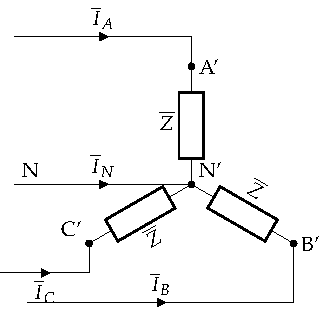
\includegraphics[width=1.05\linewidth]{../figs/EstrellaEquilibrado_Receptor.pdf}
    \end{column}
    
    \begin{column}{0.6\columnwidth}
        
        \vspace{3mm}
        Por el $\mbox{T}^{\textrm{\underline{a}}}$ de \alert{Boucherot}:

        \vspace{-6mm}
        \begin{align*}
            P &\;=\; 3 \cdot P_Z \;=\; 3 \cdot U_f\cdot I_f\cdot\cos(\theta)\\
            Q &\;=\; 3 \cdot Q_Z \;=\; 3 \cdot U_f\cdot I_f \cdot \sin(\theta)\\
        \end{align*}    
    
        \vspace{-5mm}
        Relaciones en conexión $\wye$:

        \vspace{-6mm}
        \begin{align*}
          I_f &= I_L\\
          U_f &= \frac{U_L}{\sqrt{3}}
        \end{align*}
    
        \vspace{-5mm}
        \begin{empheq}[box=\fbox]{align*}
            {\boldsymbol{\color{blue!50!black} P}} &\;=\; 3\cdot U_f \cdot I_f \cdot \cos(\theta) \;=\; \sqrt{3}\cdot  U_L \cdot I_L\cdot \cos(\theta)\\[5pt]
            {\boldsymbol{\color{blue!50!black} Q}} &\;=\; 3\cdot U_f \cdot I_f \cdot\sin(\theta) \;=\; \sqrt{3}\cdot  U_L \cdot I_L\cdot \sin(\theta)\\[5pt]
            {\boldsymbol{\color{blue!50!black} S}} &\;=\; \sqrt{P^2 + Q^2} \;=\; 3\cdot U_f\cdot I_f \;=\; \sqrt{3}\cdot U_L\cdot I_L
        \end{empheq}
    \end{column}
    \end{columns}
\end{frame}

%%%%%%%%%%%%%%%%%

\begin{frame}{Receptor en triángulo equilibrado}
    \begin{columns}
    \begin{column}{0.4\columnwidth}
        \hspace*{-11mm}
        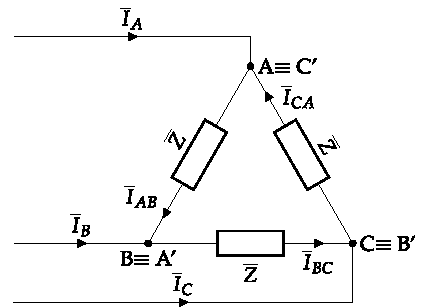
\includegraphics[width=1.2\linewidth]{../figs/TrianguloEquilibrado_Receptor.pdf}
    \end{column}
    
    \begin{column}{0.6\columnwidth}
        
        \vspace{3mm}
        Por el $\mbox{T}^{\textrm{\underline{a}}}$ de \alert{Boucherot}:

        \vspace{-6.5mm}
        \begin{align*}
            P &\;=\; 3 \cdot P_Z \;=\; 3 \cdot U_f\cdot I_f\cdot\cos(\theta)\\
            Q &\;=\; 3 \cdot Q_Z \;=\; 3 \cdot U_f\cdot I_f \cdot \sin(\theta)\\
        \end{align*}  

        \vspace{-6.5mm}
        Relaciones en conexión $\triangle$:

        \vspace{-7mm}
        \begin{align*}
          I_f &= \frac{I_L}{\sqrt{3}}\\
          U_f &= {U_L}
        \end{align*}

        \vspace{-7mm}
        \begin{empheq}[box=\fbox]{align*}
          {\boldsymbol{\color{blue!50!black} P}} & \;=\; 3\cdot U_f \cdot I_f \cdot \cos(\theta) \;=\; \sqrt{3}\cdot  U_L \cdot I_L\cdot \cos(\theta)\\[5pt]
          {\boldsymbol{\color{blue!50!black} Q}} &\;=\; 3\cdot U_f \cdot I_f \cdot \sin(\theta) \;=\; \sqrt{3}\cdot  U_L \cdot I_L\cdot \sin(\theta)\\[5pt]
          {\boldsymbol{\color{blue!50!black} S}} &\;=\; \sqrt{P^2 + Q^2} \;=\; 3\cdot U_f\cdot I_f \;=\; \sqrt{3}\cdot U_L\cdot I_L
        \end{empheq}

        \vspace{-2mm}
        \centering{\small{(\alert{mismas expresiones} que para \wye \hspace{1mm}equilibrado)}}
    \end{column}
    \end{columns}
\end{frame}

%%%%%%%%%%%%%%%%%

\begin{frame}{Receptor en estrella desequilibrado}
    \begin{columns}
    \begin{column}{0.5\columnwidth}
        \begin{center}
            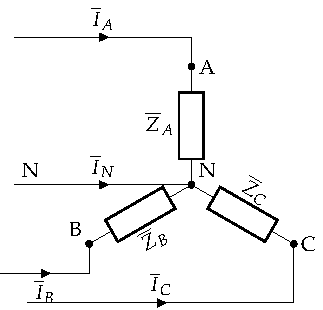
\includegraphics[width=.9\linewidth]{../figs/EstrellaDesequilibrado_Receptor.pdf}
        \end{center}
    \end{column}
    
    \begin{column}{0.5\columnwidth}
    La \alert{potencia} en cada fase puede ser \alert{distinta}, luego hay que calcular cada una y aplicar el $\mbox{T}^{\textrm{\underline{a}}}$ de Boucherot:
    
        \begin{align*}
          P &= P_{\color{red}A} + P_{\color{red}B} + P_{\color{red}C}\\[4pt]
          Q &= Q_{\color{red}A} + Q_{\color{red}B} + Q_{\color{red}C}\\[4pt]
          \overline{S} &= P + jQ
        \end{align*}
    \end{column}
    \end{columns}
\end{frame}

%%%%%%%%%%%%%%%%%

\begin{frame}{Receptor en triángulo desequilibrado} \label{diapo:triangulo_desequilibrado}
    \begin{columns}
    \begin{column}{0.5\columnwidth}
        \hspace{-5mm}
        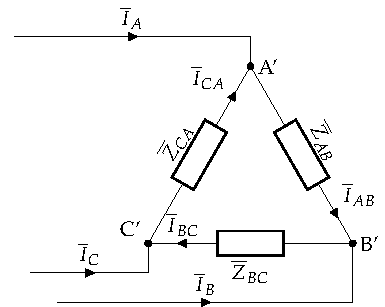
\includegraphics[width=1.05\linewidth]{../figs/TrianguloDesequilibrado_Receptor.pdf}
    \end{column}
    
    \begin{column}{0.5\columnwidth}
        La \alert{potencia} en cada fase puede ser \alert{distinta}, luego hay que calcular cada una y aplicar el $\mbox{T}^{\textrm{\underline{a}}}$ de Boucherot:
    
        \begin{align*}
          P &= P_{\color{red}AB} + P_{\color{red}BC} + P_{\color{red}CA}\\[4pt]
          Q &= Q_{\color{red}AB} + Q_{\color{red}BC} + Q_{\color{red}CA}\\[4pt]
          \overline{S} &= P + jQ
        \end{align*}
    \end{column}
    \end{columns}
\end{frame}

%%%%%%%%%%%%%%%%%

\begin{frame}{Comparativa entre monofásica y trifásica equilibrada}
    \vspace{3mm}
    Comparemos un sistema monofásico y un sistema trifásico (a 3 hilos, \textit{i.e.}, sin neutro) que transmiten la \alert{misma potencia activa} y funcionan a la \alert{misma tensión entre líneas}:
    % También el mismo factor de potencia ("theta") para la impedancia monofásica y las trifásicas
    \[
        P_{\textrm{mono}} = U \cdot I_{\textrm{mono}} \cdot \cos\theta  
        \quad = \quad\, 
        P_{\textrm{tri}} = \sqrt{3} \, U_L \cdot  I_{\textrm{tri}} \cdot \cos\theta \quad\, \rightarrow \quad\; \boxed{I_{\textrm{mono}} = \sqrt{3} \;I_{\textrm{tri}}}
    \]
    
    Las \alert{pérdidas en la línea} deben ser \alert{iguales} para salvar la \alert{misma distancia}:
    \[
      P_{\textrm{mono, línea}} = 2\cdot R_{\textrm{mono, línea}}\cdot I_{\textrm{mono}}^2 
      \quad = \quad\, 
      P_{\textrm{tri, líneas}} = 3\cdot R_{\textrm{tri, línea}}\cdot I_{\textrm{tri}}^2
    \]
    
    Sustituyendo la relación de corrientes y teniendo en cuenta la relación entre resistencia y sección (área):
    \[
      2\cdot R_{\textrm{mono, línea}} \cdot (\sqrt3\, I_{\textrm{tri}})^2 = 3\cdot R_{\textrm{tri, línea}} \cdot I_{\textrm{tri}}^2 
      \; \rightarrow \; 
      R_{\textrm{mono, línea}} = \frac{1}{2} R_{\textrm{tri, línea}} 
      \; \rightarrow \; 
      \boxed{A_{\textrm{mono}} = 2 \cdot A_{\textrm{tri}}}
    \]
    
    Finalmente, la \alert{relación} entre \alert{masas de conductor} es:    
    \[
      \frac{m_{\textrm{tri}}}{m_{\textrm{mono}}} = \frac{3 \cdot A_{\textrm{tri}}}{2 \cdot A_{\textrm{mono}}} = \frac{3}{4}
      \quad \rightarrow \quad 
      \boxed{ \;\; \vphantom{\frac{a}{a}} m_{\textrm{tri}} = 75\% \cdot m_{\textrm{mono}} \;\; }
    \]
\end{frame}

%%%%%%%%%%%%%%%

\begin{frame}{Interludio: \hspace{3mm}\textit{AC} \hspace{1mm}\textit{Optimal Power Flow}}

    \begin{itemize}
        \item Objetivo: \alert{optimizar} el coste operación de una \alert{red eléctrica}

        \vspace{2mm}        

        \fbox{ \begin{minipage}{0.35\linewidth}

            \vspace{1mm}
            
            \begin{center}
                \alert{Millones de \$} en \href{https://www.pnnl.gov/news-media/arpa-e-grid-optimization-competition-will-award-4-million-winning-software-developers}{premios}
                \vspace{0.5mm}
            \end{center}            
        \end{minipage} }
    \end{itemize}
    
    \begin{center}    
        \includegraphics[width=0.75\linewidth]{../figs/convex_nonConvex.pdf}
    \end{center}

    % Para dibujar un rectángulo blanco que tape parte de la imagen:
    \vspace{-13mm}
    
    \hspace{62.5mm}
    \begin{tikzpicture}
        \filldraw[white] (0,0) rectangle (0.3,0.3);
    \end{tikzpicture}
\end{frame}

%%%%%%%%%%%%%%%%%

\begin{frame}{Interludio: \hspace{3mm}AC-OPF, \hspace{3mm}\textit{convex} \hspace{0.5mm}\textit{relaxation}}

    \vspace{-5mm}
    
    \begin{itemize}
        \item Para \alert{minimizar} una función \alert{no convexa}, una opción $\quad \rightarrow \quad$ \textit{relajación} \hspace{0.5mm}convexa
    \end{itemize}

    \begin{columns}
    \begin{column}{0.5\columnwidth}
        \begin{center}    
            \includegraphics[width=.7\linewidth]{../figs/convexRelaxation_Tight.pdf}

            Zero relaxation gap
        \end{center}
    \end{column}
    \begin{column}{0.5\columnwidth}
        \begin{center}    
            \includegraphics[width=.7\linewidth]{../figs/convexRelaxation_nonTight.pdf}

            Non-zero relaxation gap
        \end{center}
    \end{column}
    \end{columns}

    % Para dibujar un rectángulo blanco que tape parte de la imagen:
    \vspace{-21mm}
    
    \hspace{37mm}
    \begin{tikzpicture}
        \filldraw[white] (0,0) rectangle (2.5,0.45);
    \end{tikzpicture}
\end{frame}

%%%%%%%%%%%%%%%%%

\subsection{Mejora del factor de potencia}

\begin{frame}{Mejora del factor de potencia}
    \begin{itemize}
        \item Sea un \alert{receptor equilibrado} \alert{inductivo} del que conocemos \(P\), \(Q\) y, por tanto, su factor de potencia `\(\cos \theta\)'

        \vspace{4mm}
        \item Para reducir la potencia reactiva del sistema debemos instalar un \alert{banco de condensadores} que suministrarán una potencia reactiva \(Q_c\)

        \vspace{4mm}
        \item Como resultado, la \alert{potencia reactiva} y el \alert{f.d.p.}~del sistema serán:         
        \[
            Q' = Q - Q_c  \qquad\qquad \cos\theta' > \cos \theta
        \]

        \vspace{1mm}
        \item En trifásica existen \alert{dos posibilidades}:
        
        \vspace{1mm}
        \begin{itemize}
            \normalsize
            \item Conexión en triángulo: \hspace{3mm}\(C_{\triangle}\)
            
            \vspace{2mm}
            \item Conexión en estrella: \hspace{3mm}\(C_{\wye}\)
        \end{itemize}
    \end{itemize}
\end{frame}

%%%%%%%%%%%%%%%%%

\begin{frame}{Conexión de condensadores en triángulo}
    \begin{columns}
    \begin{column}{0.5\columnwidth}
        \begin{center}
            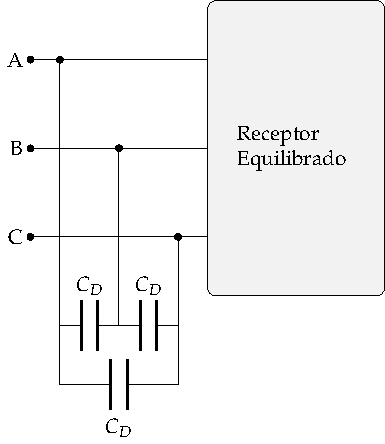
\includegraphics[width=.9\linewidth]{../figs/CircuitoTrifasica_CompensacionReactiva.pdf}
        \end{center}
    \end{column}
    
    \begin{column}{0.5\columnwidth}
        Independientemente de si el receptor está conectado en {\wye} o en $\triangle$:

        \vspace{-3mm}
        \begin{align*}
          Q &= P\cdot\tan\theta\\[4pt]
          Q' &= P\cdot\tan\theta' = Q - Q_c\\[4pt]
          Q_c &= \hspace{-4mm}\underbrace{3}_{\text{Boucherot}} \hspace{-3.5mm}\cdot \, \omega \, C_\triangle \cdot {\boldsymbol{\color{blue!50!black} U_L}}^2
        \end{align*}

        \vspace{2mm}
        \[
          \boxed{\; C_\triangle = \frac{P\cdot (\tan \theta - \tan \theta')}{\text{\Large \alert{3}} \cdot \omega \, U_L^2} \;}
        \]
    \end{column}
    \end{columns}
\end{frame}

%%%%%%%%%%%%%%%%%

\begin{frame}{Conexión de condensadores en estrella}
    \begin{columns}
    \begin{column}{0.5\columnwidth}    
    
        \vspace*{3mm}        
        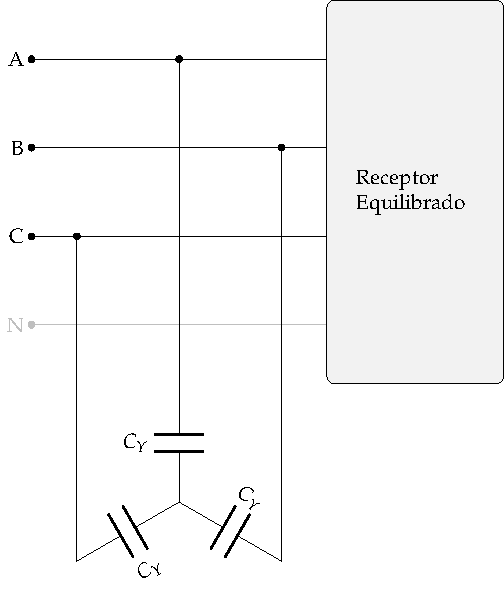
\includegraphics[width=.97\linewidth]{../figs/CircuitoTrifasicaY_CompensacionReactiva.pdf}
    \end{column}
    \begin{column}{0.5\columnwidth}    
        Independientemente de si el receptor está conectado en {\wye} o en $\triangle$:

        \vspace{-3mm}
        \begin{align*}
          Q &= P\cdot\tan\theta\\[4pt]
          Q' &= P\cdot\tan\theta' = Q - Q_c\\[4pt]
          Q_c &= \hspace{-4mm}\underbrace{3}_{\text{Boucherot}} \hspace{-3.5mm} \cdot \, \omega \, C_{\wye} \cdot {\boldsymbol{\color{blue!50!black} U_f}}^2 = \cancel{3} \cdot \omega \, C_{\wye} \cdot \left(\frac{U_L}{\cancel{\sqrt3}} \right)^2
        \end{align*}

        \vspace{2mm}
        \[
          \boxed{\; C_{\wye} = \frac{P\cdot(\tan \theta - \tan \theta')}{\omega \, U_L^2} \;}
        \]
        \begin{center}
            \small (la \alert{capacidad necesaria} en {\wye} es 
            
            \textcolor{red}{3 veces mayor} que en $\triangle$)
        \end{center}
    \end{column}
    \end{columns}
\end{frame}

%%%%%%%%%%%%%%%%%

\subsection{Medida de potencia en sistemas trifásicos}

\begin{frame}{Recordatorio: \hspace{3mm}vatímetro}
    \vspace{3mm}
    \begin{center}
        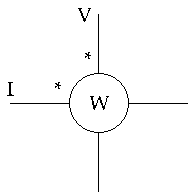
\includegraphics[height=0.5\textheight]{../figs/vatimetro.pdf}
    \end{center}

    \vspace{2mm}
    
    \centering Equipo de medida de \alert{4 terminales} (un par para tensión, un par para corriente)

    \vspace{-4mm}
    \begin{equation*}
        W 
        \; = \, 
        \underbrace{ \overline{I}\,\bullet\,\overline{U} }_{\substack{\text{producto} \\ \text{escalar}}} 
        \, = \;  
        I\cdot U\cdot \cos(\widehat{\overline{I}, \overline{U}})
        \; = \;
        \Re( \hspace{-1mm} \underbrace{\overline{U} \cdot \overline{I}^*}_{\substack{\text{potencia} \\ \text{aparente}}} \hspace{-1mm})
	\end{equation*}
    % Para escribir el "underbrace" en varias líneas: https://tex.stackexchange.com/questions/7503/how-can-i-write-multiple-lines-in-a-subscript    
\end{frame}

%%%%%%%%%%%%%%%%%

\begin{frame}{Sistema a 4 hilos (4H), \hspace{3mm} caso general}
    \begin{columns}
    \begin{column}{0.65\columnwidth}
    
        \vspace{6mm}
        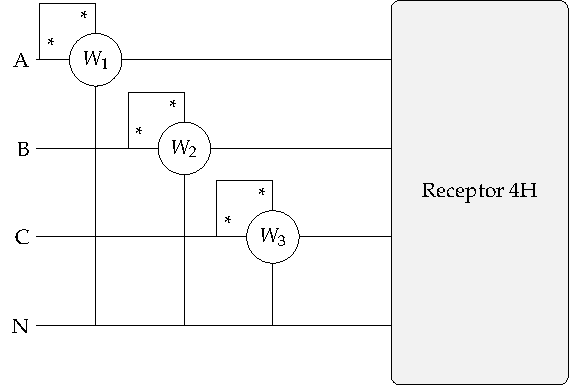
\includegraphics[height=0.75\textheight]{../figs/Potencia4H.pdf}
    \end{column}
    
    \begin{column}{0.35\columnwidth}
        En el caso general, el receptor puede ser \alert{desequilibrado} $\; \rightarrow \;$ \alert{potencia distinta} en cada fase

        \vspace{4mm}
        Son necesarios \alert{3 vatímetros}, uno por fase:
        \begin{align*}
          W_1 &= \Re(\overline{U}_A \cdot \overline{I}_A^*) = P_A\\
          W_2 &= \Re(\overline{U}_B \cdot \overline{I}_B^*) = P_B\\
          W_3 &= \Re(\overline{U}_C \cdot \overline{I}_C^*) = P_C\\
        \end{align*}

        \vspace{-2mm}
        Por el $\mbox{T}^{\textrm{\underline{a}}}$ de \alert{Boucherot}:        
        \[
          \boxed{\; P = W_1 + W_2 + W_3 \;}
        \]
    \end{column}
    \end{columns}
\end{frame}

%%%%%%%%%%%%%%%%%

\begin{frame}{Sistema a 4 hilos (4H), \hspace{3mm} caso equilibrado}
    \begin{columns}
    \begin{column}{0.45\columnwidth}
    
        \vspace{6mm}

        \hspace*{5mm}
        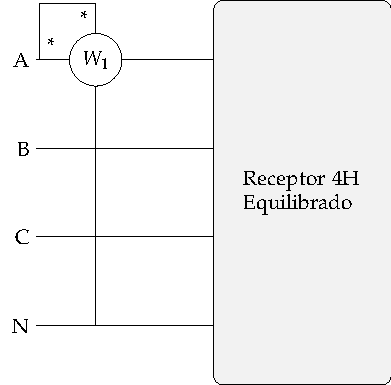
\includegraphics[height=0.75\textheight]{../figs/Potencia4H_Equilibrado.pdf}
    \end{column}
    \hfill
    \begin{column}{0.45\columnwidth}
        En el caso de un receptor \alert{equilibrado} $\; \rightarrow \;$ \alert{misma potencia} en todas las fases

        \vspace{4mm}
        Basta con \alert{1 vatímetro}:
        \[
            P_A = P_B = P_C
        \]

        \vspace{2mm}
        Por el $\mbox{T}^{\textrm{\underline{a}}}$ de \alert{Boucherot}:        
        \[
            \boxed{\; P = 3 \cdot W_1 \;}
        \]
    \end{column}
    \end{columns}
\end{frame}

%%%%%%%%%%%%%%%%%

\begin{frame}{Sistema a 3 hilos (3H)}

    \vspace{2mm}
    \textcolor{red}{NO} es posible usar \textcolor{red}{3 vatímetros}, porque no es posible medir $P$ en cada $Z$ \alert{por separado}:
    
    \begin{itemize}
        \item Si el \alert{receptor} está conectado en $\wye$: no es posible medir la \alert{tensión de fase}

        \vspace{1mm}
        \item Si el \alert{receptor} está conectado en $\triangle$: no es posible medir la \alert{corriente de fase}
    \end{itemize}
    
    \begin{columns}
    \begin{column}{0.44\linewidth}

        \vspace{4mm}

        \hspace*{-3mm}
        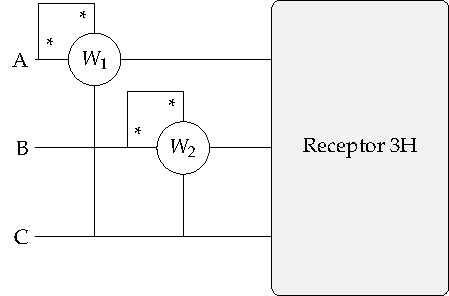
\includegraphics[width=1\linewidth]{../figs/Potencia3H.pdf}
    \end{column}
    \begin{column}{0.53\linewidth}

        \vspace{2mm}
        Pero \alert{existe un método} para medida de potencia en sistemas a 3 hilos

        \vspace{1mm}
        \begin{itemize}
            \item Válido tanto para receptores en $\wye$ como 
            
            en $\triangle$, equilibrados o desequilibrados
        \end{itemize}

        \vspace{2mm}
        
        \centering
        
        \fbox{ \begin{minipage}{0.8\linewidth}

            \vspace{1mm}
            
            \begin{center}
                El ``método de los \alert{2 vatímetros}'', 
                
                o ``montaje de \alert{Aron}''
                \vspace{0.5mm}
            \end{center}            
        \end{minipage} }

        \vspace{-2mm}
        \[ 
            \boxed{\; P = W_1+W_2 \;}
        \]

        \small{(demostración a continuación)}
    \end{column}
    \end{columns}
\end{frame}

%%%%%%%%%%%%%%%%%

\begin{frame}{Método de los 2 vatímetros: \hspace{3mm}demostración}

    \vspace{2mm}
    Para un \alert{receptor} en $\wye$    
    \hspace{3mm}(sin asumir que sea necesariamente equilibrado)

    \vspace{2mm}
    \alert{Potencia total} en el receptor: 

    \vspace{-4mm}
    \begin{equation*}
	    \overline{S}
        \; = \; 
        \overline{S}_A + \overline{S}_B + \overline{S}_C
        \; = \; 
        \overline{U}_A \cdot \overline{I}_A^* + \overline{U}_B \cdot \overline{I}_B^* + \overline{U}_C \cdot \overline{I}_C^*
	\end{equation*}
 
	\begin{columns}
	\begin{column}{0.6\linewidth}
    
        Al no haber conductor neutro (\alert{3 hilos}), por \alert{1LK} en 
        
        el punto común de la $\wye$:
    	\begin{equation*}
    	    \overline{I}_A + \overline{I}_B + \overline{I}_C = 0 
            \quad \rightarrow \quad 
            \overline{I}_C = -(\overline{I}_A+\overline{I}_B)
    	\end{equation*}
    	Sustituyendo en la $1^{\textrm{a}}$ expresión y agrupando términos:
        \begin{equation*}
            \overline{S}
            \; = \;
            \overline{U}_{AC} \cdot \overline{I}_A^* + \overline{U}_{BC} \cdot \overline{I}_B^*
        \end{equation*} 

        \vspace{-2mm}
        \begin{equation*}
            P 
            \; = \;
            \Re(\overline{U}_{AC} \cdot \overline{I}_A^* + \overline{U}_{BC} \cdot \overline{I}_B^* )
            \; = \;
            \boxed{\; W_1 + W_2 \;}
        \end{equation*}  
	\end{column}
 
	\begin{column}{0.4\linewidth}

        \vspace*{8mm}
        
        \hspace*{-8mm}
        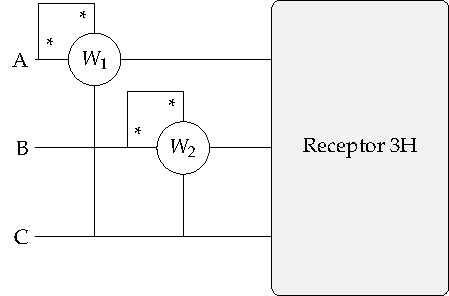
\includegraphics[width=1.1\linewidth]{../figs/Potencia3H.pdf}
	\end{column}
	\end{columns}
\end{frame}

%%%%%%%%%%%%%%%%%

\begin{frame}{Método de los 2 vatímetros: \hspace{3mm}demostración}

    \vspace{2mm}
    Para un \alert{receptor} en $\triangle$    
    \hspace{3mm}(sin asumir que sea necesariamente equilibrado)

    \vspace{0.5mm}
    \alert{Potencia total} 
    \(  \quad \rightarrow \quad\;
        \overline{S}
        \; = \; 
        \overline{S}_{AB} + \overline{S}_{BC} + \overline{S}_{CA}
        \; = \; 
        \overline{U}_{AB} \cdot \overline{I}_{AB}^* + \overline{U}_{BC} \cdot \overline{I}_{BC}^* + \overline{U}_{CA} \cdot \overline{I}_{CA}^*
    \)

    \vspace{2mm}
	\begin{columns}
	\begin{column}{0.6\linewidth}
    
        Aplicando \alert{2LK} en el $\triangle$ del \hyperlink{diapo:triangulo_desequilibrado}{receptor}:
        \begin{equation*}
    	    \overline{U}_{AB} + \overline{U}_{BC} + \overline{U}_{CA} = 0 
            \;\, \rightarrow \;\, 
            \overline{U}_{AB} = -(\overline{U}_{BC} + \overline{U}_{CA})
    	\end{equation*}

        y aplicando \alert{1LK} en los nudos del \hyperlink{diapo:triangulo_desequilibrado}{receptor}:

        \vspace{-2mm}
    	\begin{equation*}
    	    \overline{I}_{CA} = \overline{I}_{AB} - \overline{I}_A \; , 
            \quad 
            \overline{I}_{BC} = \overline{I}_B + \overline{I}_{AB}
    	\end{equation*}

    	Sustituyendo en la $1^{\textrm{a}}$ expresión y agrupando:

        \vspace{-2mm}
        \begin{equation*}
            \overline{S}
            \; = \;
            \overline{U}_{AC} \cdot \overline{I}_A^* + \overline{U}_{BC} \cdot \overline{I}_B^*
        \end{equation*} 

        \vspace{-3mm}
        \begin{equation*}
            P 
            \; = \;
            \Re(\overline{U}_{AC} \cdot \overline{I}_A^* + \overline{U}_{BC} \cdot \overline{I}_B^* )
            \; = \;
            \boxed{\; W_1 + W_2 \;}
        \end{equation*}  

        \centering
        \small{(\alert{mismo resultado} que en $\wye$)}
	\end{column}
 
	\begin{column}{0.4\linewidth}

        \vspace*{13mm}
        
        \hspace*{-8mm}
        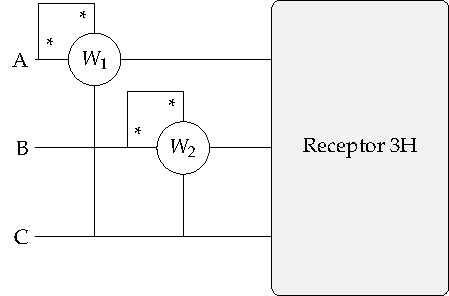
\includegraphics[width=1.1\linewidth]{../figs/Potencia3H.pdf}
	\end{column}
	\end{columns}
\end{frame}

%%%%%%%%%%%%%%%%%

\begin{frame}{Resumen, \hspace{3mm}medida de potencia en sistemas trifásicos}
    \vspace{-1mm}
    \[
      \begin{array}{lc}
        \text{Conexión del receptor} & \;\; \text{N° de vatímetros necesarios}\\[5pt]
        \hline\\[-5pt]
        \minibox[l]{\wye \hspace{1.5mm}a 4 hilos (\alert{con} neutro), \\[0pt] equilibrado} & 1 \\[20pt]
        \minibox[l]{\wye \hspace{1.5mm}a 4 hilos (\alert{con} neutro), \\[0pt] \alert{des}equilibrado} & 3\\[20pt]
        \minibox[l]{\wye \hspace{1.5mm}a 3 hilos (\alert{sin} neutro), \\[0pt] equilibrado o \alert{des}equilibrado} & \minibox[l]{\hspace{13.7mm} 2 \\[0pt] (montaje de Aron)}\\[20pt]
        \minibox[l]{\ensuremath{\triangle} equilibrado o \alert{des}equilibrado, \\[0pt] (\ensuremath{\triangle} implica 3 hilos)} & \minibox[l]{\hspace{13.7mm} 2 \\[0pt] (montaje de Aron)}
      \end{array}
    \]
    % "Minibox", para poder partir el texto en 2 líneas: https://tex.stackexchange.com/questions/8680/how-can-i-insert-a-newline-in-a-framebox
    % Sobre "\smash{\raisebox", sacado de aquí: https://tex.stackexchange.com/questions/153225/combining-rows-and-columns-in-array
\end{frame}

%%%%%%%%%%%%%%%%%

\begin{frame}{Método de los 2 vatímetros, caso particular: \hspace{3mm}receptor equilibrado}
    \vspace{2mm}
    \begin{itemize}
        \item En el caso particular de un \alert{receptor equilibrado}, el método de los 2 vatímetros aporta \alert{información adicional} $\quad \rightarrow \quad$ también permite medir \alert{potencia reactiva}

        \vspace{2mm}
        \item Para demostrarlo, consideramos un \alert{receptor} de carácter \alert{inductivo}, tanto en \alert{SFD} como en \alert{SFI} \hspace{3mm}(ver siguientes 2 diapositivas)
    \end{itemize}    

    \begin{center}
        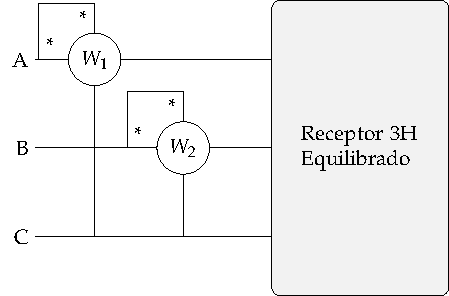
\includegraphics[width=.53\linewidth]{../figs/Potencia_3H_equilibrado_AB.pdf}
    \end{center}
\end{frame}

%%%%%%%%%%%%%%%%%

\begin{frame}{Método de los 2 vatímetros: \hspace{3mm}receptor equilibrado, \hspace{3mm}SFD}
    \begin{columns}
    \begin{column}{0.5\columnwidth}

        \vspace{3mm}
        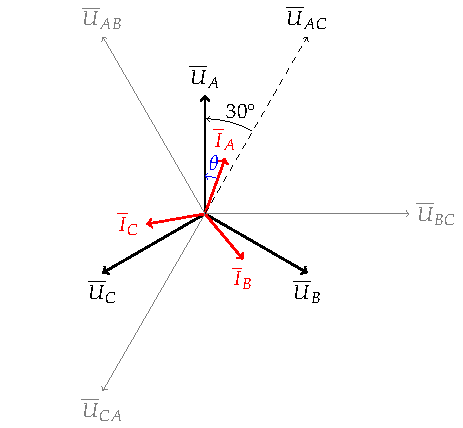
\includegraphics[height=0.9\textheight]{../figs/fasores_potencia3H.pdf}
    \end{column}
    \begin{column}{0.5\columnwidth}    
        \begin{align*}
    	    W_1& 
            \;=\; 
            \overline{U}_{AC}\,\bullet\,\overline{I}_A
            \;=\;
            U_L \cdot I_L \cdot \overbrace{\cos(30^\circ - \theta)}^{\text{ver gráfico}}\\[7pt] 
    	    W_2& 
            \;=\; 
            \overline{U}_{BC}\,\bullet\,\overline{I}_B
            \;=\;
            U_L \cdot I_L \cdot \underbrace{\cos(30^\circ + \theta)}_{\text{ver gráfico}}
    	\end{align*}

        \hspace{3mm}Usando \href{https://raw.githubusercontent.com/ETSIDI-IE/tc/master/docs/diapos/TC1_Trigonometria_Complejos_LBB.pdf}{$\cos(\alpha-\beta)$} se llega a:
        
    	\[
            \boxed{\; W_1 + W_2
            \;=\; \sqrt3 \, U_L \, I_L \, \cos \theta 
            \;=\; P \;}
        \]

        \[
            \boxed{\; W_1 \, {\Large\boldsymbol{\color{blue!50!black} -}} \, W_2
            \;=\; U_L \, I_L \, \sin \theta 
            \;=\; \frac{Q}{\boldsymbol{\color{blue!50!black} \sqrt{3}}} \;}
        \]        
    \end{column}
    \end{columns}
\end{frame}

%%%%%%%%%%%%%%%%%

\begin{frame}{Método de los 2 vatímetros: \hspace{3mm}receptor equilibrado, \hspace{3mm}SFI}
    \begin{columns}
    \begin{column}{0.5\columnwidth}

        \vspace{3mm}
        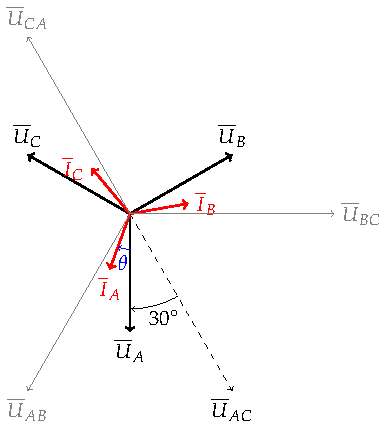
\includegraphics[height=0.9\textheight]{../figs/fasores_potencia3H_SFI.pdf}
    \end{column}
    \begin{column}{0.5\columnwidth} 

        \vspace{-3mm}
        Los únicos \textcolor{red}{cambios} para \alert{SFI} son:

        \vspace{-7mm}
        \begin{align*}
    	    W_1& 
            \;=\; 
            \overline{U}_{AC}\,\bullet\,\overline{I}_A
            \;=\;
            U_L \cdot I_L \cdot \overbrace{\cos(\color{red}{30^\circ + \theta}\color{black}{)}}^{\text{ver gráfico}}\\[7pt] 
    	    W_2& 
            \;=\; 
            \overline{U}_{BC}\,\bullet\,\overline{I}_B
            \;=\;
            U_L \cdot I_L \cdot \underbrace{\cos(\color{red}{30^\circ - \theta}\color{black}{)}}_{\text{ver gráfico}}
    	\end{align*}

        \hspace{3mm}Usando \href{https://raw.githubusercontent.com/ETSIDI-IE/tc/master/docs/diapos/TC1_Trigonometria_Complejos_LBB.pdf}{$\cos(\alpha-\beta)$} se llega a:
        
    	\[
            \boxed{\; W_1 + W_2
            \;=\; \sqrt3 \, U_L \, I_L \, \cos \theta 
            \;=\; P \;}
        \]

        \vspace{-4mm}
        \[
            \boxed{\; W_1 \, {\Large\boldsymbol{\color{blue!50!black} -}} \, W_2
            \;=\, {\Large\boldsymbol{\color{red} -}} \, U_L \, I_L \, \sin \theta 
            \;=\, {\Large\boldsymbol{\color{red} -}} \, \frac{Q}{\boldsymbol{\color{blue!50!black} \sqrt{3}}} \;}
        \]        
    \end{column}
    \end{columns}
\end{frame}

%%%%%%%%%%%%%%%%%

\begin{frame}{Método de los 2 vatímetros: \hspace{3mm}receptor equilibrado, \hspace{3mm}otras conexiones} \label{diapo:2vat_reglaMnemotecnica}

    \vspace{1mm}
    Aunque hasta ahora hemos considerado que $W_1$ mide la tensión $U_{AC}$ y $W_2$ la tensión $U_{BC}$, existen \alert{3 posibilidades de conexión} para el método de los 2 vatímetros
    
    Para aplicar las expresiones ya vistas para $P$ y $Q$ en cualquier conexión, usamos esta \alert{regla mnemotécnica}: 
    \begin{itemize}
        \item ${\boldsymbol{\color{blue!50!black} W_1}}$ mide una \alert{tensión que} ${\boldsymbol{\color{blue!50!black} \cancel{\in}}}$ al sistema de fases
        \item ${\boldsymbol{\color{blue!50!black} W_2}}$ mide una \alert{tensión que} ${\boldsymbol{\color{blue!50!black} \in}}$ al sistema de fases
    \end{itemize}

    \centering\small{(en las 2 siguientes diapositivas se define cuándo una tensión ``pertenece'' al sistema de fases)}
    
    \begin{columns}
    \begin{column}{0.33\columnwidth}
        \begin{center}
            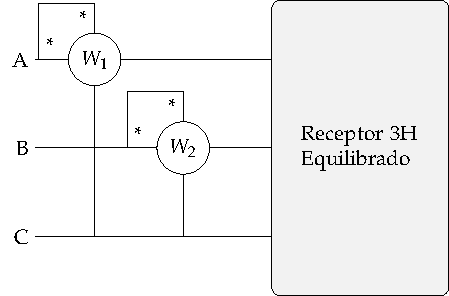
\includegraphics[width=1\linewidth]{../figs/Potencia_3H_equilibrado_AB.pdf}
        \end{center}
    \end{column}
    \begin{column}{0.33\columnwidth}
        \begin{center}
            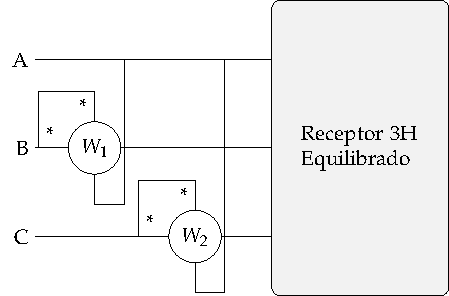
\includegraphics[width=1\linewidth]{../figs/Potencia_3H_equilibrado_BC.pdf}
        \end{center}
    \end{column}    
    \begin{column}{0.33\columnwidth}
        \begin{center}
            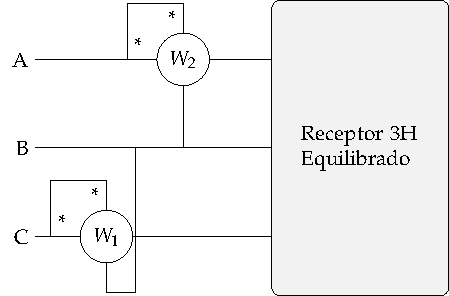
\includegraphics[width=1\linewidth]{../figs/Potencia_3H_equilibrado_CA.pdf}
        \end{center}
    \end{column}
    \end{columns}
\end{frame}

%%%%%%%%%%%%%%%%%

\begin{frame}{Otras conexiones de vatímetros, \hspace{3mm}SFD}

    \vspace{2mm}
    La tensiones que ``pertenecen'' a \alert{SFD} son:

    \vspace{-4mm}
    \[
      \boxed{(\hyperlink{diapo:secuencias_fases}{ABC}): A \triangleright B \triangleright C \Longrightarrow \{AB, BC, CA\}}
    \]

    \vspace{-2mm}
    \[
      P = W_1 + W_2\qquad \qquad Q = {\boldsymbol{\color{blue!50!black} \sqrt{3}}} \, (W_1 - W_2)
    \]
    
    \begin{columns}
    \begin{column}{0.33\columnwidth}
        \begin{center}
            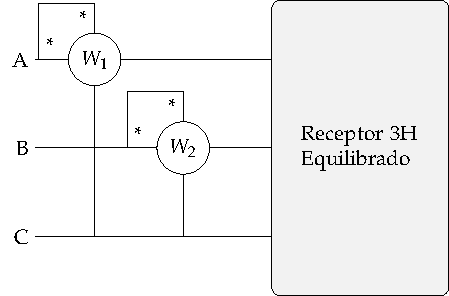
\includegraphics[width=1\linewidth]{../figs/Potencia_3H_equilibrado_AB.pdf}
        \end{center}

        \vspace{-8mm}
        \begin{align*}
          {\boldsymbol{\color{blue!50!black} W_1}}&: AC \notin \text{SFD}\\
          {\boldsymbol{\color{blue!50!black} W_2}}&: BC \in \text{SFD}
        \end{align*}
    \end{column}
    \begin{column}{0.33\columnwidth}
        \begin{center}
            \includegraphics[width=1\linewidth]{../figs/Potencia_3H_equilibrado_BC.pdf}
        \end{center}

        \vspace{-8mm}
        \begin{align*}
          {\boldsymbol{\color{blue!50!black} W_1}}&: BA \notin \text{SFD}\\
          {\boldsymbol{\color{blue!50!black} W_2}}&: CA \in \text{SFD}
        \end{align*}
    \end{column}    
    \begin{column}{0.33\columnwidth}
        \begin{center}
            \includegraphics[width=1\linewidth]{../figs/Potencia_3H_equilibrado_CA.pdf}
        \end{center}

        \vspace{-8mm}
        \begin{align*}
          {\boldsymbol{\color{blue!50!black} W_1}}&: CB \notin \text{SFD}\\
          {\boldsymbol{\color{blue!50!black} W_2}}&: AB \in \text{SFD}
        \end{align*}
    \end{column}
    \end{columns}
\end{frame}

%%%%%%%%%%%%%%%%%

\begin{frame}{Otras conexiones de vatímetros, \hspace{3mm}SFI}

    \vspace{2mm}
    La tensiones que ``pertenecen'' a \alert{SFI} son:

    \vspace{-4mm}
    \[
      \boxed{(\hyperlink{diapo:secuencias_fases}{ACB}): A \triangleright C \triangleright B \Longrightarrow \{AC, CB, BA\}}
    \]

    \vspace{-2mm}
    \[
      P = W_1 + W_2\qquad \qquad Q = {\boldsymbol{\color{blue!50!black} \sqrt{3}}} \, (W_1 - W_2)
    \]
    
    \begin{columns}
    \begin{column}{0.33\columnwidth}
        \begin{center}
            \includegraphics[width=1\linewidth]{../figs/Potencia3H_Equilibrado_AB_SFI.pdf}
        \end{center}
        
        \vspace{-8mm}
        \begin{align*}
          {\boldsymbol{\color{blue!50!black} W_1}}&: BC \notin \text{SFI}\\
          {\boldsymbol{\color{blue!50!black} W_2}}&: AC \in \text{SFI}\\
        \end{align*}
    \end{column}
    \begin{column}{0.33\columnwidth}
        \begin{center}
            \includegraphics[width=1\linewidth]{../figs/Potencia3H_Equilibrado_BC_SFI.pdf}
        \end{center}
        
        \vspace{-8mm}
        \begin{align*}
          {\boldsymbol{\color{blue!50!black} W_1}}&: CA \notin \text{SFI}\\
          {\boldsymbol{\color{blue!50!black} W_2}}&: BA \in \text{SFI}\\
        \end{align*}
    \end{column}
    \begin{column}{0.33\columnwidth}
        \begin{center}
            \includegraphics[width=1\linewidth]{../figs/Potencia3H_Equilibrado_CA_SFI.pdf}
        \end{center}
        
        \vspace{-8mm}
        \begin{align*}
          {\boldsymbol{\color{blue!50!black} W_1}}&: AB \notin \text{SFI}\\
          {\boldsymbol{\color{blue!50!black} W_2}}&: CB \in \text{SFI}\\
        \end{align*}
    \end{column}
    \end{columns}
\end{frame}

%%%%%%%%%%%%%%%%%

\begin{frame}{Medida de reactiva con 1 vatímetro \hspace{3mm}(sistemas equilibrados)}
    
    \vspace{2mm}
    \begin{itemize}
        \item En el caso particular de un \alert{receptor equilibrado} a 3 hilos, también es posible medir \alert{potencia reactiva} con un único vatímetro

        \vspace{2mm}
        \item Para demostrarlo, consideramos un \alert{receptor} de carácter \alert{inductivo}, tanto en \alert{SFD} como en \alert{SFI} \hspace{3mm}(ver siguientes 2 diapositivas)
    \end{itemize}    

    \begin{center}
        \includegraphics[width=.45\linewidth]{../figs/Reactiva3H_A-BC.pdf}
    \end{center}
\end{frame}

%%%%%%%%%%%%%%%%%

\begin{frame}{Medida de reactiva con 1 vatímetro, \hspace{3mm}SFD}
    \begin{columns}
    \begin{column}{0.5\columnwidth}

        \vspace{3mm}
        \includegraphics[height=0.9\textheight]{../figs/fasores_potencia3H_reactiva.pdf}
    \end{column}
    \begin{column}{0.5\columnwidth}    
        \begin{equation*}
    	    W 
            \;=\; 
            \overline{U}_{BC}\,\bullet\,\overline{I}_A
            \;=\;
            U_L \cdot I_L \cdot \overbrace{\cos(90^\circ - \theta)}^{\text{ver gráfico}}
    	\end{equation*}

        \vspace{10mm}
        
        \hspace{3mm}Usando \href{https://raw.githubusercontent.com/ETSIDI-IE/tc/master/docs/diapos/TC1_Trigonometria_Complejos_LBB.pdf}{$\cos(\alpha-\beta)$} se llega a:
        
        \[
            \boxed{\; W
            \;=\; U_L \, I_L \, \sin \theta 
            \;=\; \frac{Q}{\boldsymbol{\color{blue!50!black} \sqrt{3}}} \;}
        \]        
    \end{column}
    \end{columns}
\end{frame}

%%%%%%%%%%%%%%%%%

\begin{frame}{Medida de reactiva con 1 vatímetro, \hspace{3mm}SFI}
    \begin{columns}
    \begin{column}{0.5\columnwidth}

        \vspace{3mm}
        \includegraphics[height=0.9\textheight]{../figs/fasores_potencia3H_SFI_reactiva.pdf}
    \end{column}
    \begin{column}{0.5\columnwidth}    
        El único \textcolor{red}{cambio} para \alert{SFI} es:

        \vspace{-7mm}
        \begin{equation*}
    	    W 
            \;=\; 
            \overline{U}_{BC}\,\bullet\,\overline{I}_A
            \;=\;
            U_L \cdot I_L \cdot \overbrace{\cos(90^\circ \color{red}{+} \, \color{black}{\theta)}}^{\text{ver gráfico}}
    	\end{equation*}

        \vspace{10mm}
        
        \hspace{3mm}Usando \href{https://raw.githubusercontent.com/ETSIDI-IE/tc/master/docs/diapos/TC1_Trigonometria_Complejos_LBB.pdf}{$\cos(\alpha-\beta)$} se llega a:
        
        \[
            \boxed{\; W
            \;=\, 
            {\Large\boldsymbol{\color{red} -}} \, U_L \, I_L \, \sin \theta 
            \;=\,
            {\Large\boldsymbol{\color{red} -}} \, \frac{Q}{\boldsymbol{\color{blue!50!black} \sqrt{3}}} \;}
        \]        
    \end{column}
    \end{columns}
\end{frame}

%%%%%%%%%%%%%%%%%

\begin{frame}{Medida de reactiva con 1 vatímetro, \hspace{3mm}otras conexiones} \label{diapo:1vat_reactiva_1}
    \begin{columns}
    \begin{column}{0.33\columnwidth}
        \begin{center}
            \includegraphics[width=.9\linewidth]{../figs/Reactiva3H_A-BC.pdf}
        \end{center}

        \vspace{-10mm}
        \begin{align*}
          BC &\in \text{SFD}\\
          BC &\notin \text{SFI}
        \end{align*}
    \end{column}
    \begin{column}{0.33\columnwidth}
        \begin{center}
            \includegraphics[width=.9\linewidth]{../figs/Reactiva3H_B-CA.pdf}
        \end{center}

        \vspace{-10mm}
        \begin{align*}
          CA &\in \text{SFD}\\
          CA &\notin \text{SFI}
        \end{align*}
    \end{column}
    \begin{column}{0.33\columnwidth}
        \begin{center}
            \includegraphics[width=.9\linewidth]{../figs/Reactiva3H_C-AB.pdf}
        \end{center}

        \vspace{-10mm}
        \begin{align*}
          AB &\in \text{SFD}\\
          AB &\notin \text{SFI}
        \end{align*}
    \end{column}
    \end{columns}
    \begin{align*}
        \text{SFD} & \;\rightarrow\; \boxed{\; W \;=\; \frac{Q}{\boldsymbol{\color{blue!50!black} \sqrt{3}}} \;}\\[3pt]
        \text{SFI} & \;\rightarrow\; \boxed{\; W \;=\,  {\Large\boldsymbol{\color{red} -}} \, \frac{Q}{\boldsymbol{\color{blue!50!black} \sqrt{3}}} \;}
    \end{align*}
\end{frame}

%%%%%%%%%%%%%%%%%

\begin{frame}{Medida de reactiva con 1 vatímetro, \hspace{3mm}otras conexiones} \label{diapo:1vat_reactiva_2}
    \begin{columns}
    \begin{column}{0.33\columnwidth}
        \begin{center}
            \includegraphics[width=.9\linewidth]{../figs/Reactiva3H_A-CB.pdf}
        \end{center}

        \vspace{-10mm}
        \begin{align*}
          CB &\notin \text{SFD}\\
          CB &\in \text{SFI}
        \end{align*}
    \end{column}
    \begin{column}{0.33\columnwidth}
        \begin{center}
            \includegraphics[width=.9\linewidth]{../figs/Reactiva3H_B-AC.pdf}
        \end{center}

        \vspace{-10mm}
        \begin{align*}
          AC &\notin \text{SFD}\\
          AC &\in \text{SFI}
        \end{align*}
    \end{column}
    \begin{column}{0.33\columnwidth}
        \begin{center}
            \includegraphics[width=.9\linewidth]{../figs/Reactiva3H_C-BA.pdf}
        \end{center}

        \vspace{-10mm}
        \begin{align*}
          BA &\notin \text{SFD}\\
          BA &\in \text{SFI}
        \end{align*}
    \end{column}
    \end{columns}
    \begin{align*}
        \text{SFD} & \;\rightarrow\; \boxed{\; W \;=\, {\Large\boldsymbol{\color{red} -}} \, \frac{Q}{\boldsymbol{\color{blue!50!black} \sqrt{3}}} \;}\\[3pt]
        \text{SFI} & \;\rightarrow\; \boxed{\; W \;=\; \frac{Q}{\boldsymbol{\color{blue!50!black} \sqrt{3}}} \;}
    \end{align*}
\end{frame}

%%%%%%%%%%%%%%%%%

\begin{frame}{Resumen, \hspace{3mm}potencia en receptores \underline{equilibrados} a 3 hilos}

    \vspace{3mm}

    \fbox{ \begin{minipage}{0.58\linewidth}

        \vspace{1mm}
        
        \begin{center}
            Método de los \alert{2 vatímetros} (o ``montaje de Aron'')
            \vspace{0.5mm}
        \end{center}            
    \end{minipage} }

    \begin{adjustwidth}{0.5cm}{} % Necesita "\usepackage{changepage}"
    \begin{itemize}
        \normalsize

        \item Permite medir $\; {\boldsymbol{\color{blue!50!black} P}} \;\,$ y $\; {\boldsymbol{\color{blue!50!black} \dfrac{Q}{\sqrt3}}}$ \hspace{3mm}(\underline{importante} recordar el factor $\sqrt3$ en $Q$)

        \vspace{3mm}
        \item \textcolor{red}{Cuidado} con el \alert{signo} de ${\boldsymbol{\color{blue!50!black} Q}}$\hspace{0.2mm}:

        \vspace{1mm}
        depende de la \alert{conexión} de los vatímetros y de la \alert{secuencia de fases} (SFD o SFI)

        \vspace{1mm}
        (regla mnemotécnica \hyperlink{diapo:2vat_reglaMnemotecnica}{aquí})
    \end{itemize}
    \end{adjustwidth}

    \vspace{2mm}
    
    \fbox{ \begin{minipage}{0.42\linewidth}

        \vspace{1mm}
        
        \begin{center}
            Medida de \alert{reactiva} con \alert{1 vatímetro}
            \vspace{1mm}
        \end{center}            
    \end{minipage} }
    \begin{adjustwidth}{0.5cm}{}
    \begin{itemize}
        \normalsize

        \vspace{1mm}
        \item Debe medir \alert{una corriente de línea} y la \alert{tensión entre las otras dos} líneas

        \vspace{2mm}
        \item \underline{Importante} recordar el factor ${\boldsymbol{\color{blue!50!black} \sqrt3}}$ en ${\boldsymbol{\color{blue!50!black} Q}}$ 

        \vspace{2mm}
        \item \textcolor{red}{Cuidado} con el \alert{signo} de ${\boldsymbol{\color{blue!50!black} Q}}$\hspace{0.2mm}: 

        \vspace{1mm}
        depende de la \alert{conexión} y de la \alert{secuencia de fases} \hspace{3mm}(ver diapositivas~\ref{diapo:1vat_reactiva_1} y \ref{diapo:1vat_reactiva_2})
    \end{itemize}
    \end{adjustwidth}
\end{frame}

%%%%%%%%%%%%%%%

\begin{frame}{Interludio: \hspace{3mm}corriente continua de alta tensión \hspace{3mm}(\textit{HVDC})}
    \begin{minipage}[c]{0.49\linewidth} 
        
        \vspace{-2.75mm}
        \begin{itemize}
            \item Más \alert{económica} que corriente alterna para \alert{largas distancias} 
            
            o \alert{cables submarinos}
        \end{itemize}

        \vspace{1mm}
        \begin{center}    
            \includegraphics[width=0.9\linewidth]{../figs/costHVDC.png}
        \end{center}
    \end{minipage}
    \hfill%
    \begin{minipage}[c]{0.49\linewidth}
    
        \vspace{5mm}
        \begin{itemize}
            \item Proyecto \href{https://xlinks.co/morocco-uk-power-project/}{Xlinks}: 
            
            $3{.}800$\,\si{\kilo\meter} de cables submarinos HVDC
        \end{itemize}

        \vspace{-4mm}
        \begin{center}    
            \includegraphics[width=0.9\linewidth]{../figs/HVDC_Xlinks.jpg}
        \end{center}
    \end{minipage}
\end{frame}

\end{document}
